\newpage
\section{Progettazione}

\subsection{Progettazione Architetturale}

\subsubsection{Requisiti non funzionali}

Dall'analisi dei requisiti sono emersi i seguenti requisiti non funzionali:
\begin{itemize}
    \item Tempo di risposta
    \item Usabilità
    \item Affidabilità
    \item Scalabilità
    \item Integrità dei dati
    \item Protezione dei dati
    \item Sicurezza delle comunicazioni
\end{itemize}

L'affidabilità e la scalabilità assumono fondamentale importanza vista la natura del software,
che deve permettere agli utenti di poter organizzare, coordinare e condividere eventi.
La compromissione di questi risulterebbe in un peggioramento dell'esperienza utente, da cui consegue una perdita di reputazione o di fedeltà del cliente.
Sarà necessario assicurare la sicurezza fisica dei dati immagazzinati nel sistema, così come la sicurezza software dei dati e delle comunicazioni.
In caso di compromissione la perdita d'immagine e i risvolti legali sarebbero significativi.
L'utilizzo di protocolli e tecnologie standard del settore dovrebbero garantire la sicurezza del sitema senza peggiorarne significativamente l'usabilità o le prestazioni.
Nonostante il sistema non presenti vincoli di tempo stringenti, una caratteristica essenziale dell'applicazione sarà la velocità di distribuire gli aggiornamenti ai vari utenti.
Inoltre, l'intuitività dell'interfaccia è fondamentale per l'usabilità e la diffusione del prodotto.

\subsubsection{Scelte tecnologiche}

La scelta tecnologica principale ricade sul tipo di applicazione che si andrà a
sviluppare.
In questo caso la scelta è quella di sviluppare sia un'interfaccia per browser web, sia un'applicazione per dispositivo mobile, per i seguenti motivi:
\begin{enumerate}
    \item un'interfaccia web consente di avere una
          piattaforma standard accessibile da quasi tutti i dispositivi, con il solo
          requisito di un browser, potenzialmente permettendo(in base alla dimensione dello schermo) una maggior facilità di utilizzo, per rispondere all'esigenza organizzativa di medio o lungo termine.
          In questo modo si evita di restringere le possibilità di accesso al servizio.
    \item  l'applicazione mobile permette una gestione a breve termine e un aggiornamento costante, ed è fondamentale per recuperare le immagini dell'utente.
\end{enumerate}
\newpage
\subsubsection{Scelta dell'architettura}

Dopo una rapida analisi, si è constatato che l'architettura più adeguata per il
sistema è l'\textbf{architettura client-server a 3 livelli}.

\paragraph{L1 -- Client}\mbox{}\\
La componente lato Client implementerà l'interfaccia utente, gestendo le interazioni del cliente e richiedendo i dati al server,
salvandoli in una cache locale laddove la tecnologia lo renda possibile. Inoltre avrà la responsabilità di recuperare le immagini scattate durante l'evento.

\paragraph{L2 -- Server}\mbox{}\\
Per distribuire meglio il carico, si è deciso di scomporre i server in base alle funzionalità offerte. Si hanno quindi tre server:

\begin{itemize}
    \item[-] Un server per le funzionalità di autenticazione
    \item[-] Un server principale che fornisce i servizi agli utenti
    \item[-] Un server che gestisce la propagazione degli aggiornamenti agli utenti
\end{itemize}

\paragraph{L3 -- Persistenza}\mbox{}\\
La gestione della persistenza verrà implementata in due server con responsabilità differenti:
\begin{itemize}
    \item[-] Un server sul quale sarà installato un DBMS relazionale che gestisca i dati e le relazioni dei componenti
    \item[-] Un server per il salvataggio delle immagini e file
\end{itemize}

Il database relazionale sarà accessibile solo dal server che fornisce i servizi, per garantire il controllo dei ruoli e dei permessi.
Le immagini saranno invece accessibili solo in lettura direttamente dai client, che dovranno però essere a conoscenza dei codici che le identificano.
Questa conoscenza è considerata sufficente per garantire la confidenza, ammesso che l'identificativo sia lungo abbastanza,
ma anche un rischio accettabile, in quanto ridurrà di molto il carico del server principale.

\subsubsection{Pattern architetturali e di design}

Il pattern Client-Server è stato scelto come pattern architetturale per gestire l'accesso, le immagini e i servizi principali.\\
Il pattern Event Driven sarà invece usato per notificare i Client degli aggiornamenti.
A livello di design distinguiamo tre componenti principali: Model, View e Controller.
Mentre la View sarà delegata completamente ai Client, Model e Controller saranno invece suddivisi tra il Client e il Server,
in base alle necessità di caching dei dati e della località delle operazioni di business.\\
Si riportano di seguito i diagrammi di package e componenti che descrivono l'architettura del sistema.\\
TODO accesso to DB

\newpage
\begin{figure}[h!]
    \begin{center}
        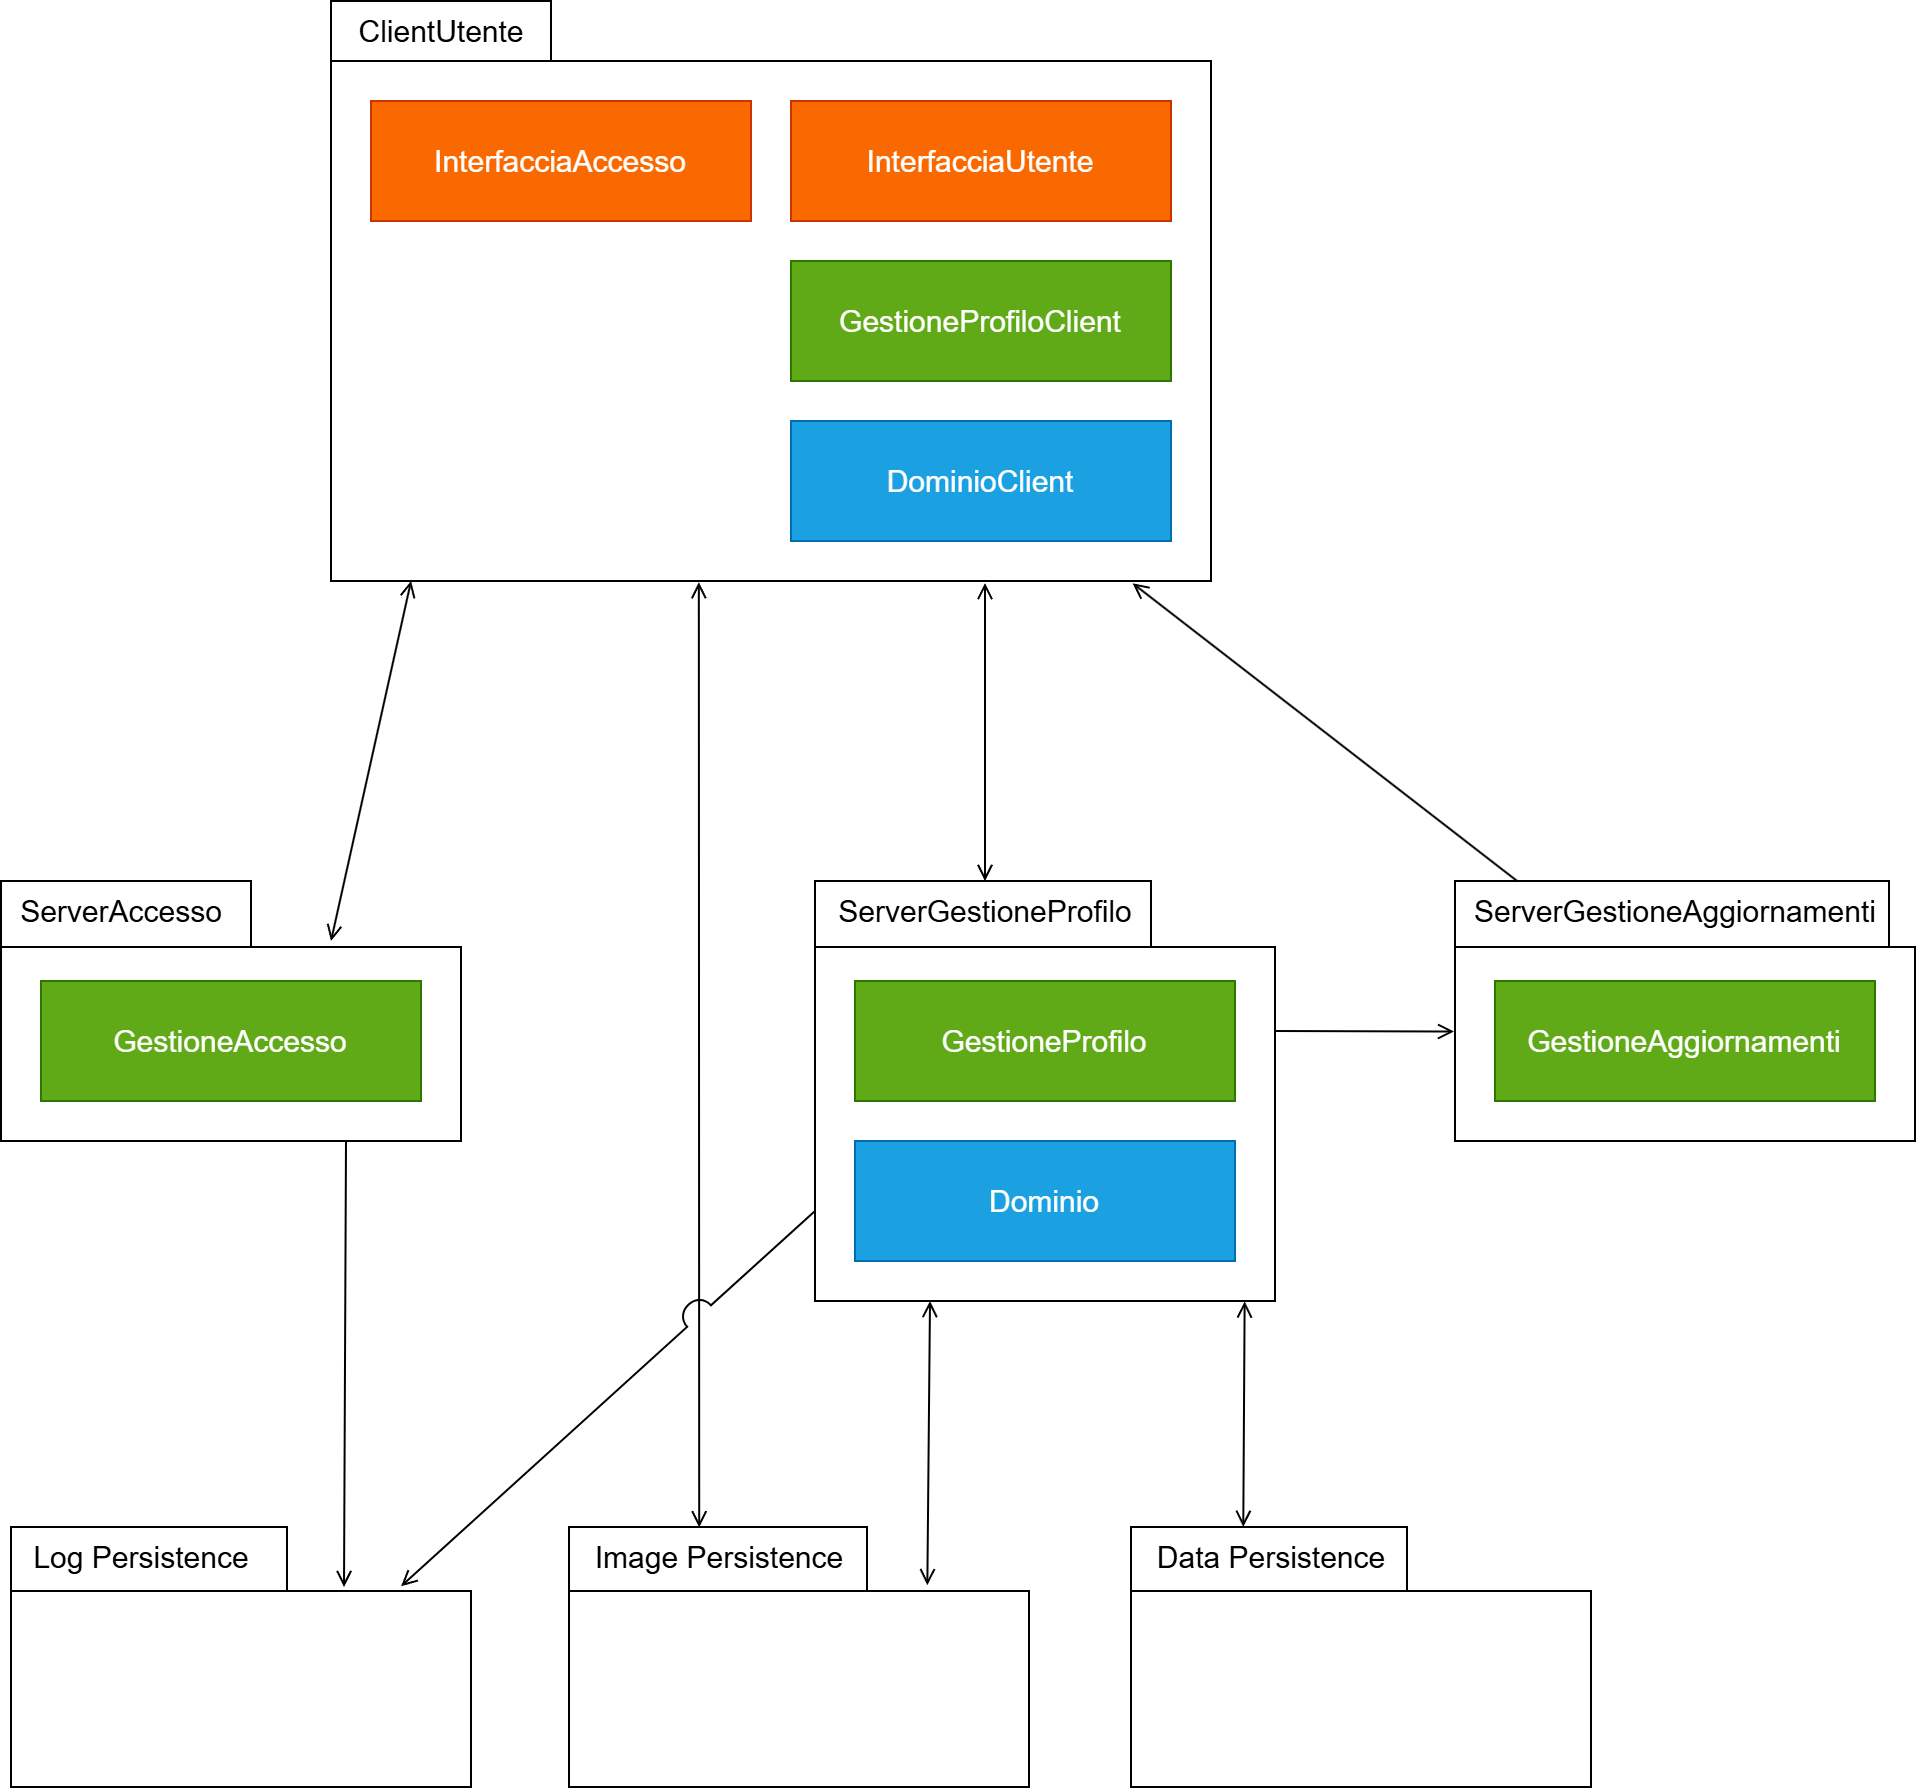
\includegraphics[height=0.5\textheight]{ProgettoDiagrammaPackage.png}
        \caption{Diagramma dei package}
    \end{center}
\end{figure}

\begin{figure}[h!]
    \begin{center}
        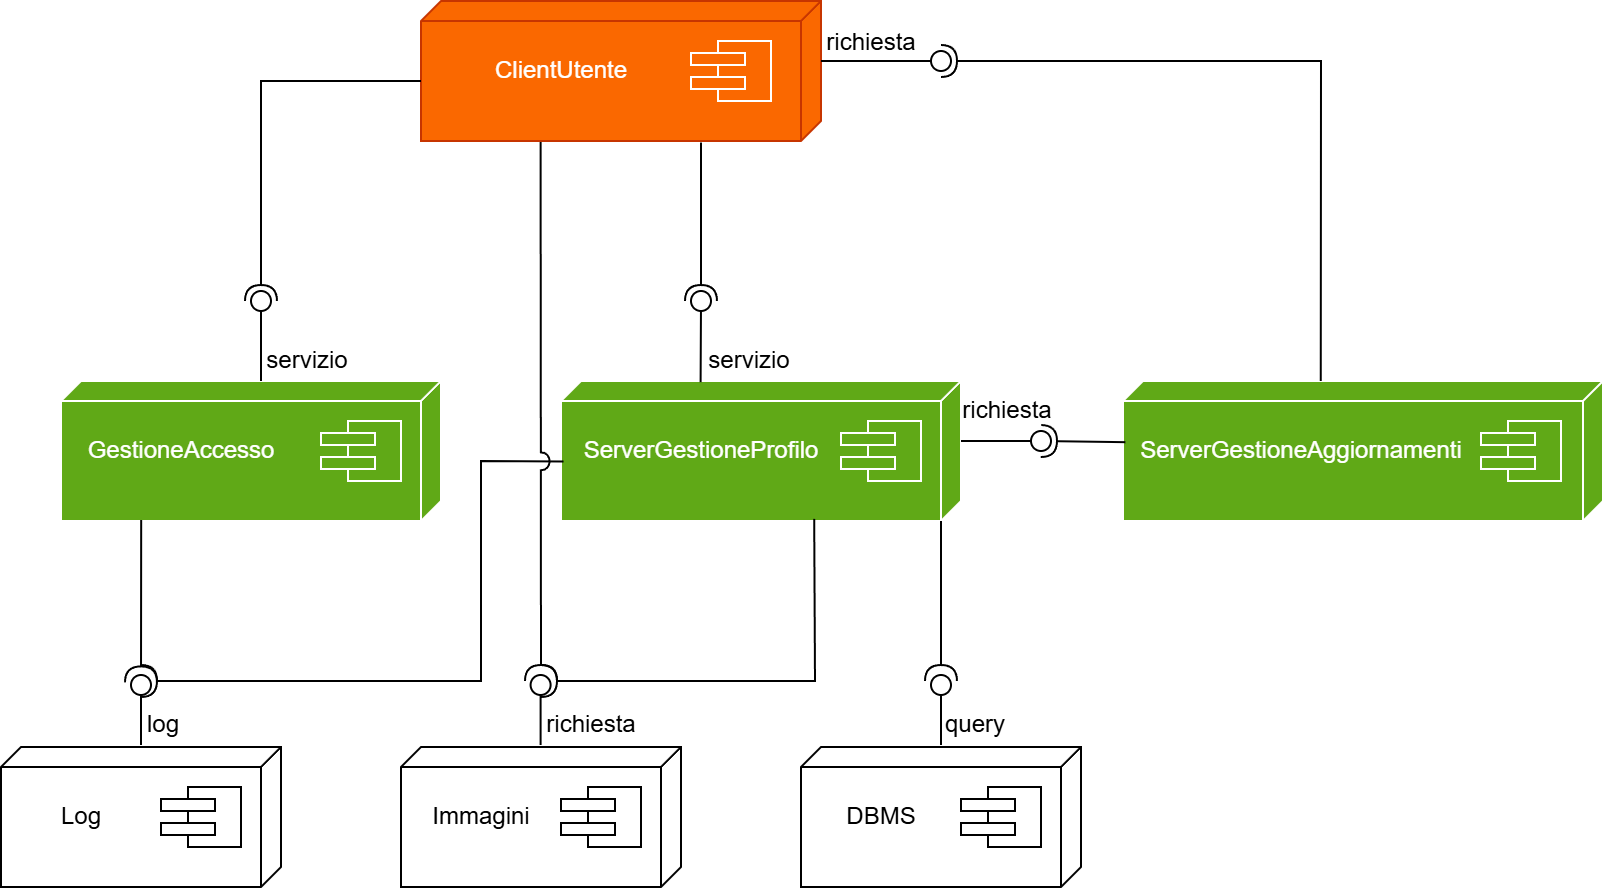
\includegraphics[height=0.3\textheight]{ProgettoDiagrammaComponenti.png}
        \caption{Diagramma dei componenti}
    \end{center}
\end{figure}

\newpage

\subsection{Progettazione di dettaglio}

\subsubsection{Struttura: Dominio}

Per quanto riguarda il dominio, distinguiamo il dominio del server dal dominio del client.

\vspace{1em}

\textbf{Diagramma di dettaglio: Dominio Server}\\
Aggiungiamo a tutti i componenti principali un identificativo anfanumerico chiamato hash,
e le date di creazione e di ultima modifica per gestire meglio i log e gli aggiornamenti.
Inoltre, aggiungiamo un componente per definire il ruolo dell'utente sul profilo.
\begin{figure}[h!]
    \begin{center}
        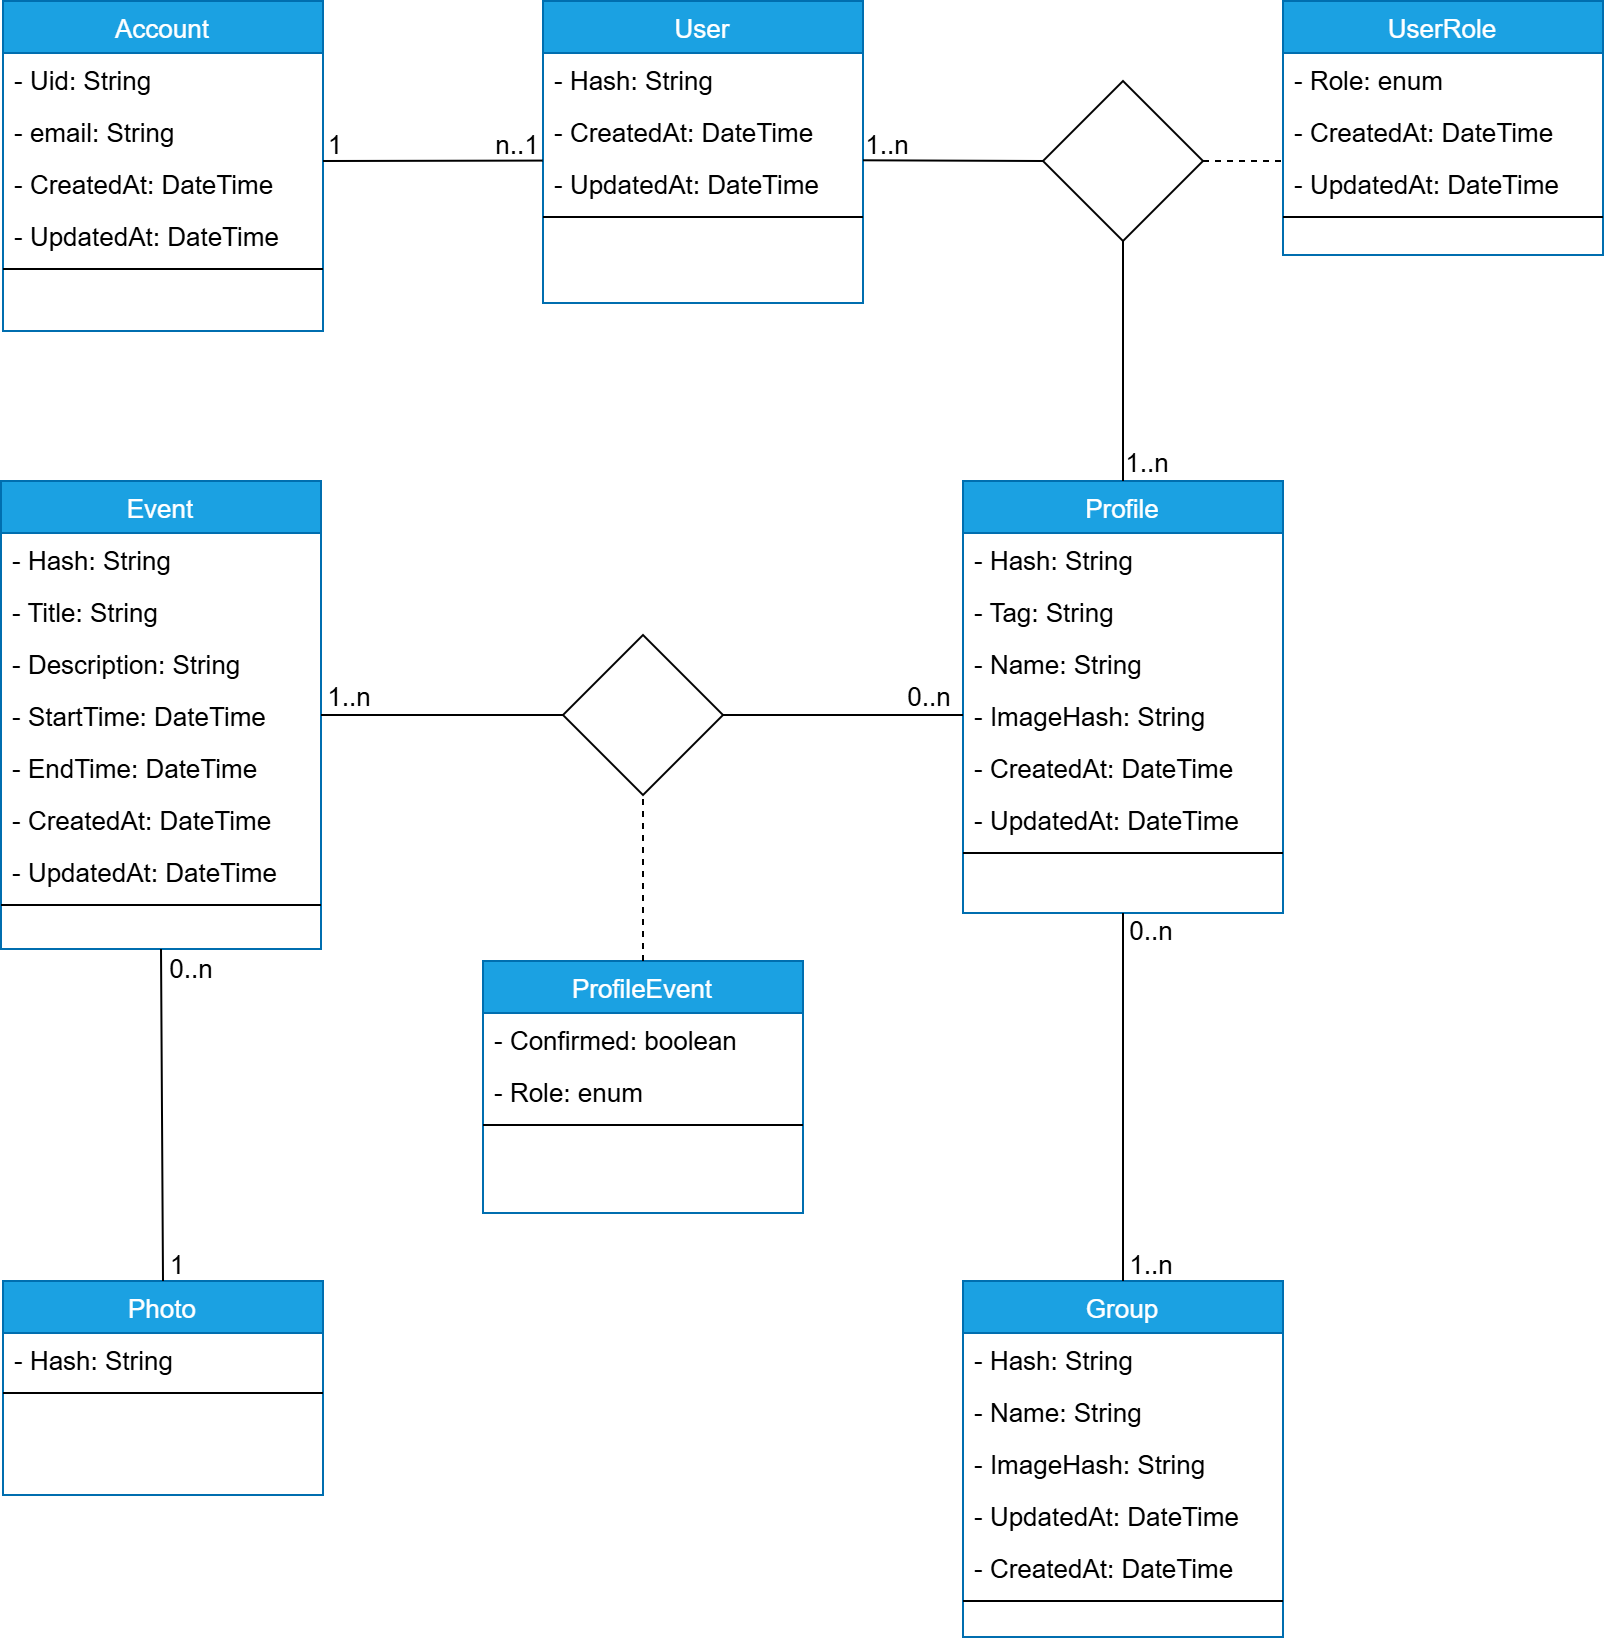
\includegraphics[width=\textwidth]{ProgettoDominioServer.png}
    \end{center}
\end{figure}

\newpage

\textbf{Diagramma di dettaglio: Dominio Client}\\
Dal punto di vista del client alcune relazioni non sono più rilevanti o vengono semplificate integrando alcuni valori all'interno di altri elementi del dominio.
\begin{figure}[h!]
    \begin{center}
        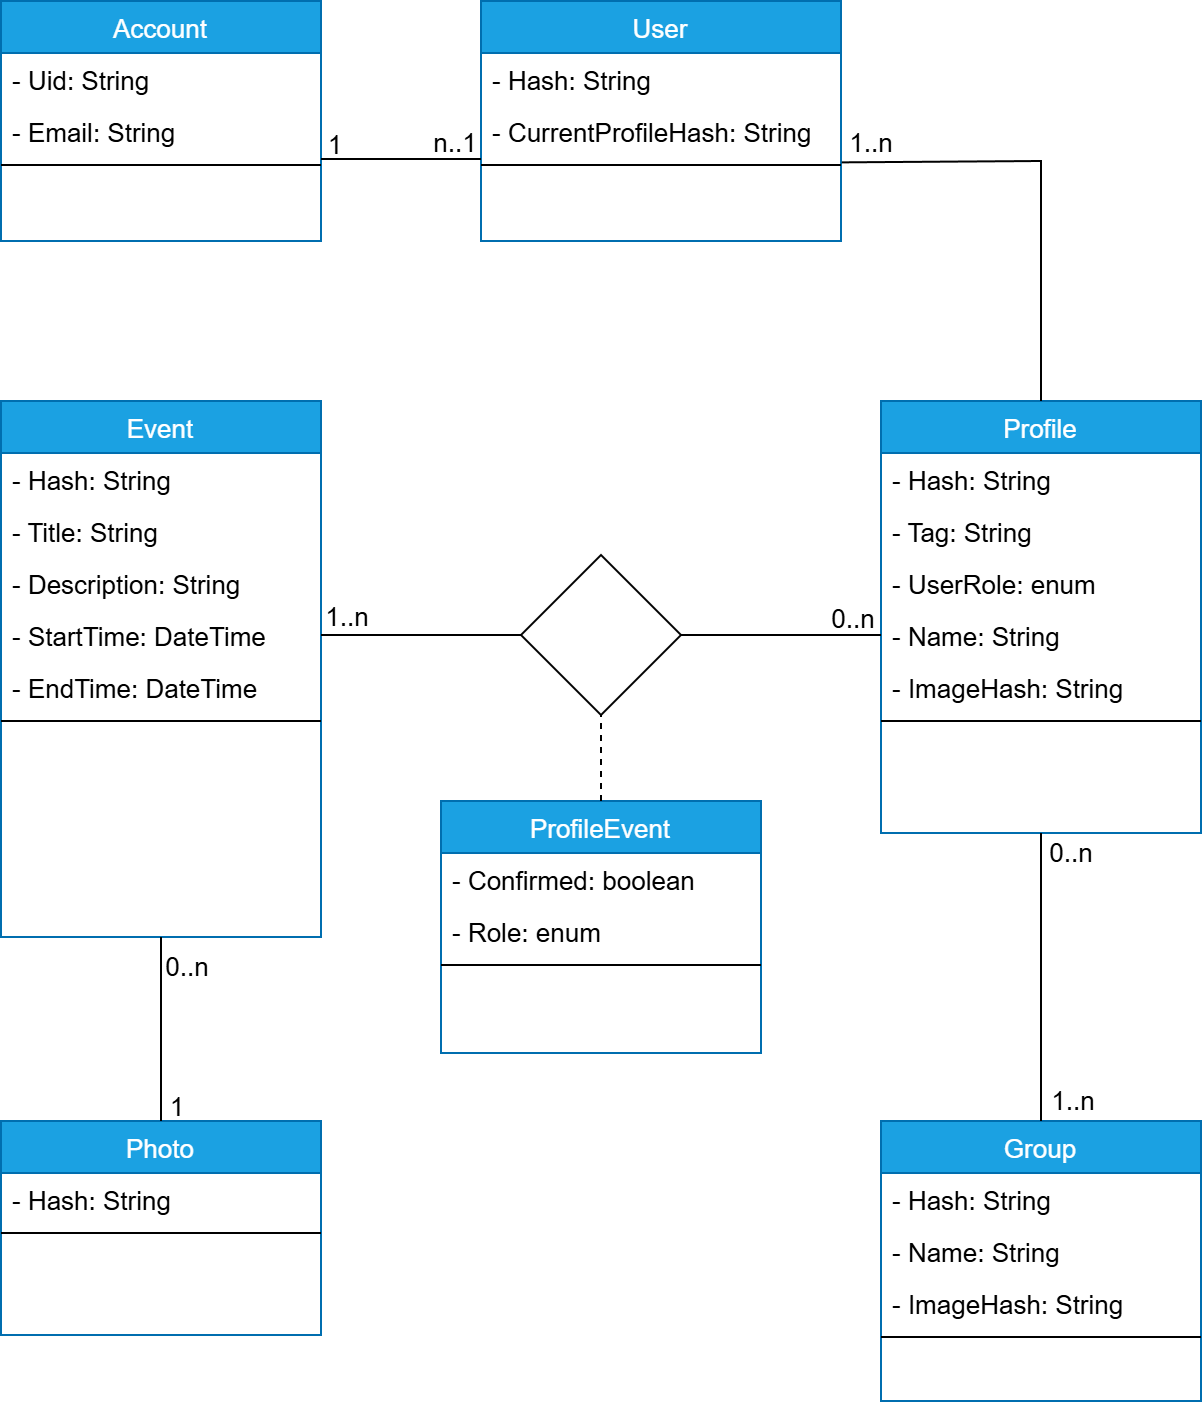
\includegraphics[width=\textwidth]{ProgettoDominioClient.png}
    \end{center}
\end{figure}
\clearpage

\subsubsection{Struttura: Interfacce}

\textbf{Diagramma di dettaglio: Interfacce Gestione Accesso e Gestione Aggiornamenti}
\begin{figure}[h!]
    \begin{center}
        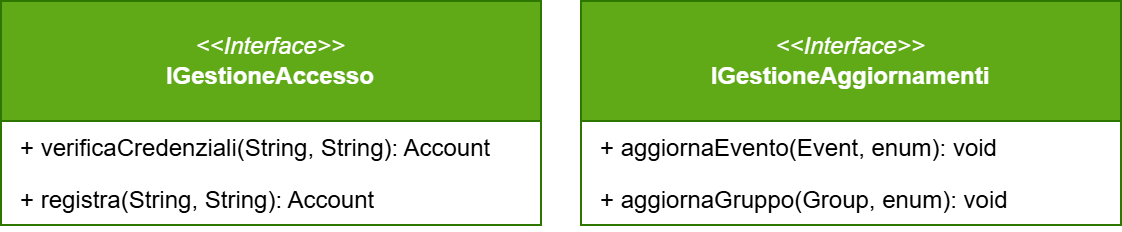
\includegraphics[height=0.09\textheight]{ProgettoInterfacceAccesso.png}
    \end{center}
\end{figure}

\textbf{Diagramma di dettaglio: Interfacce Client}
\begin{figure}[h!]
    \begin{center}
        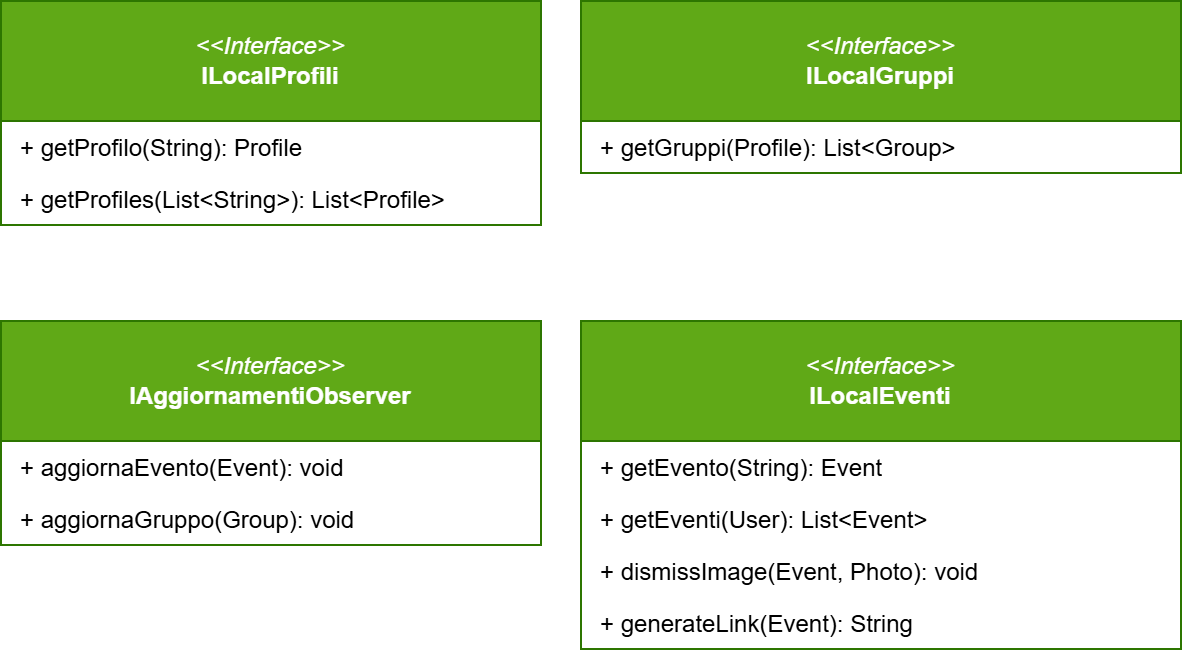
\includegraphics[height=0.24\textheight]{ProgettoInterfacceClient.png}
    \end{center}
\end{figure}

\textbf{Diagramma di dettaglio: Interfacce Server}
\begin{figure}[h!]
    \begin{center}
        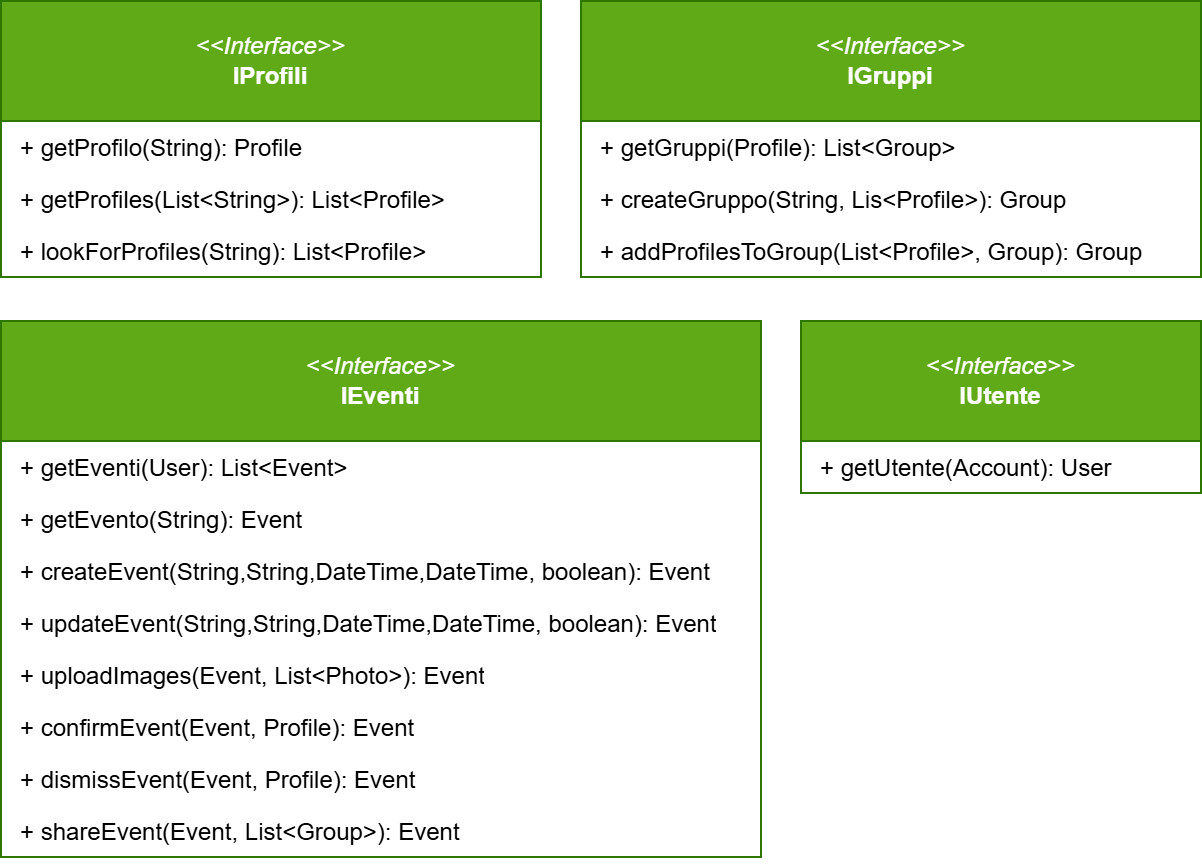
\includegraphics[height=0.31\textheight]{ProgettoInterfacceServer.png}
    \end{center}
\end{figure}\\

Le interfacce client e server risultano molto simili in quanto il client, prima di fare una richiesta dati al server, controllerà la cache locale per cercare i dati.
L'aggiunta di tali interfacce consente di applicare il \textit{Dependency Inversion Principle}
in modo da disaccoppiare gli utilizzatori dalle implementazioni, che potrebbero cambiare.

\clearpage

\subsubsection{Struttura: Controller}

Ogni interfaccia verrà implementata da un relativo controller.
\vspace{1em}

\textbf{Diagramma di dettaglio: Gestione Accesso e Gestione Aggiornamenti}
\\Introduciamo un Controller per la connessione con la persistenza del log
\begin{figure}[h!]
    \begin{center}
        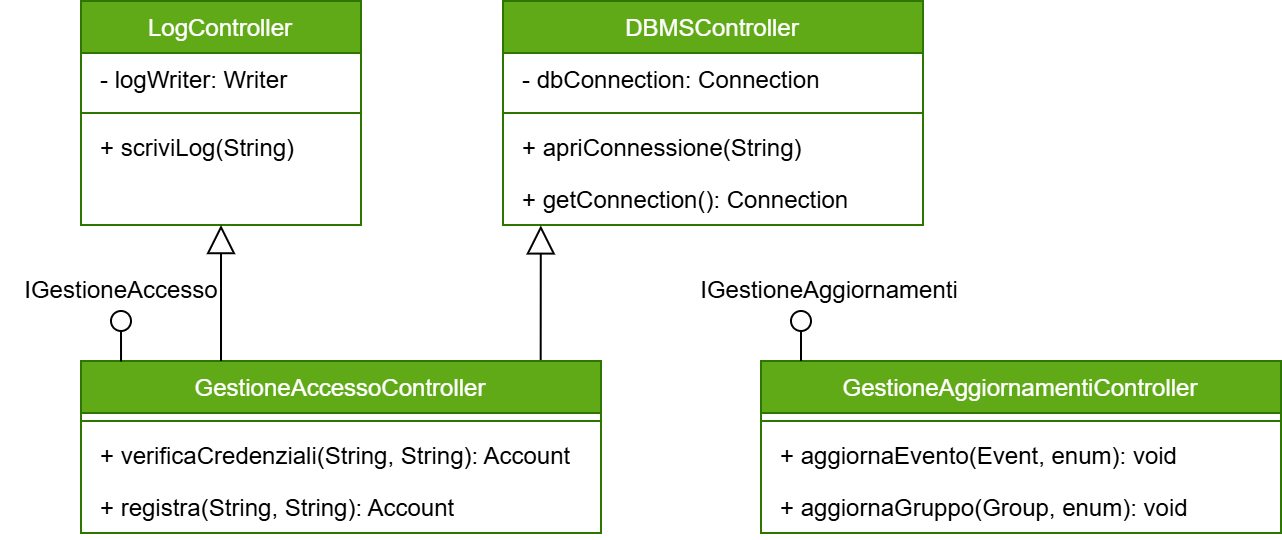
\includegraphics[height=0.25\textheight]{ProgettoControllerAccesso.png}
    \end{center}
\end{figure}

\textbf{Diagramma di dettaglio: Client}
\begin{figure}[h!]
    \begin{center}
        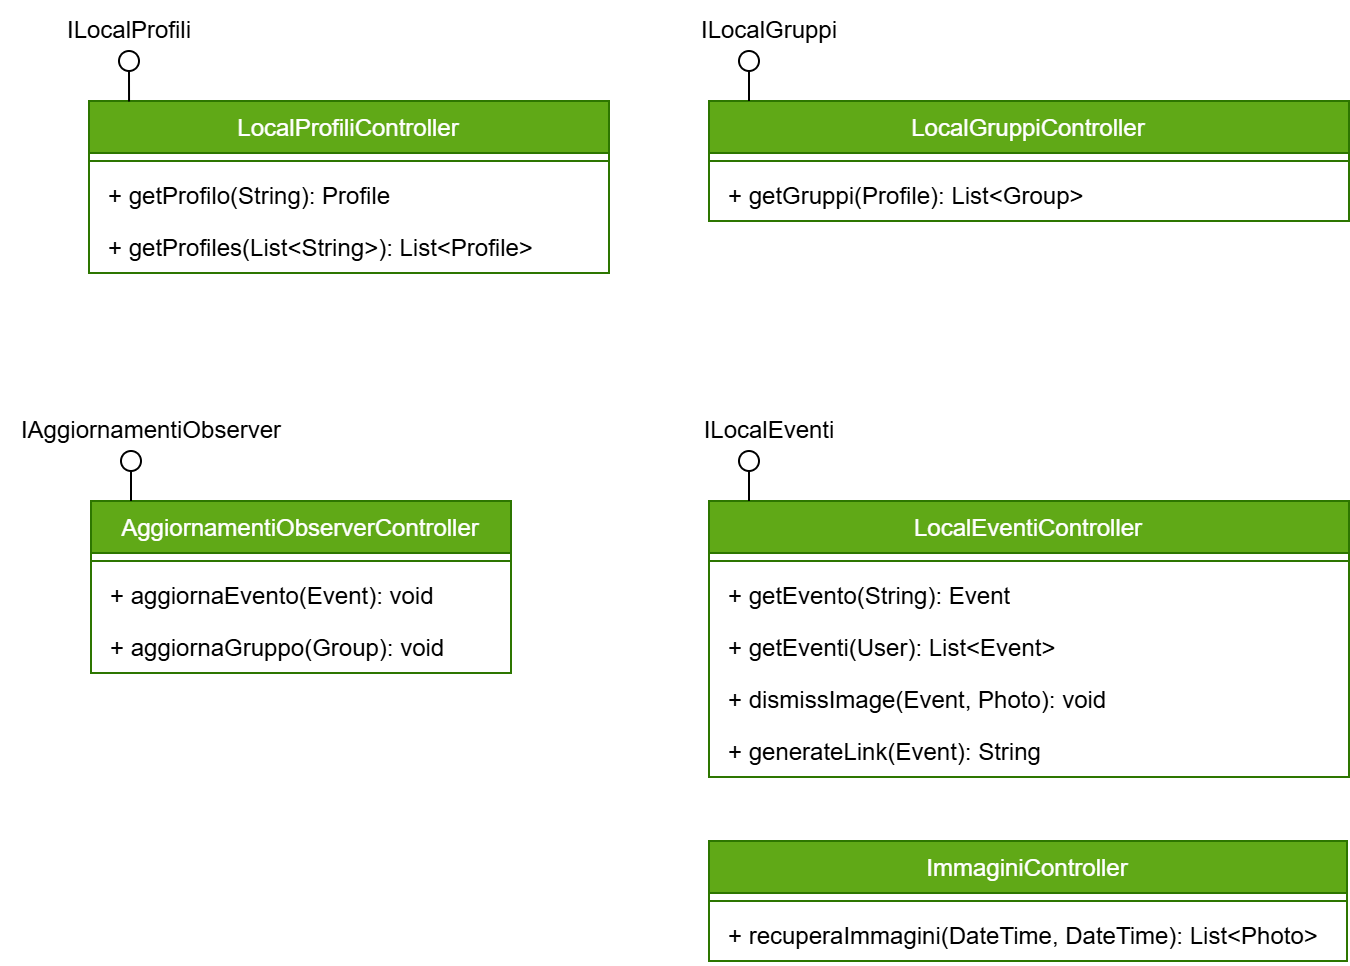
\includegraphics[height=0.45\textheight]{ProgettoControllerClient.png}
    \end{center}
\end{figure}


\clearpage

\subsubsection{Struttura: Interfacce Grafiche}

\textbf{Diagramma di dettaglio: Server}
\begin{figure}[h!]
    \begin{center}
        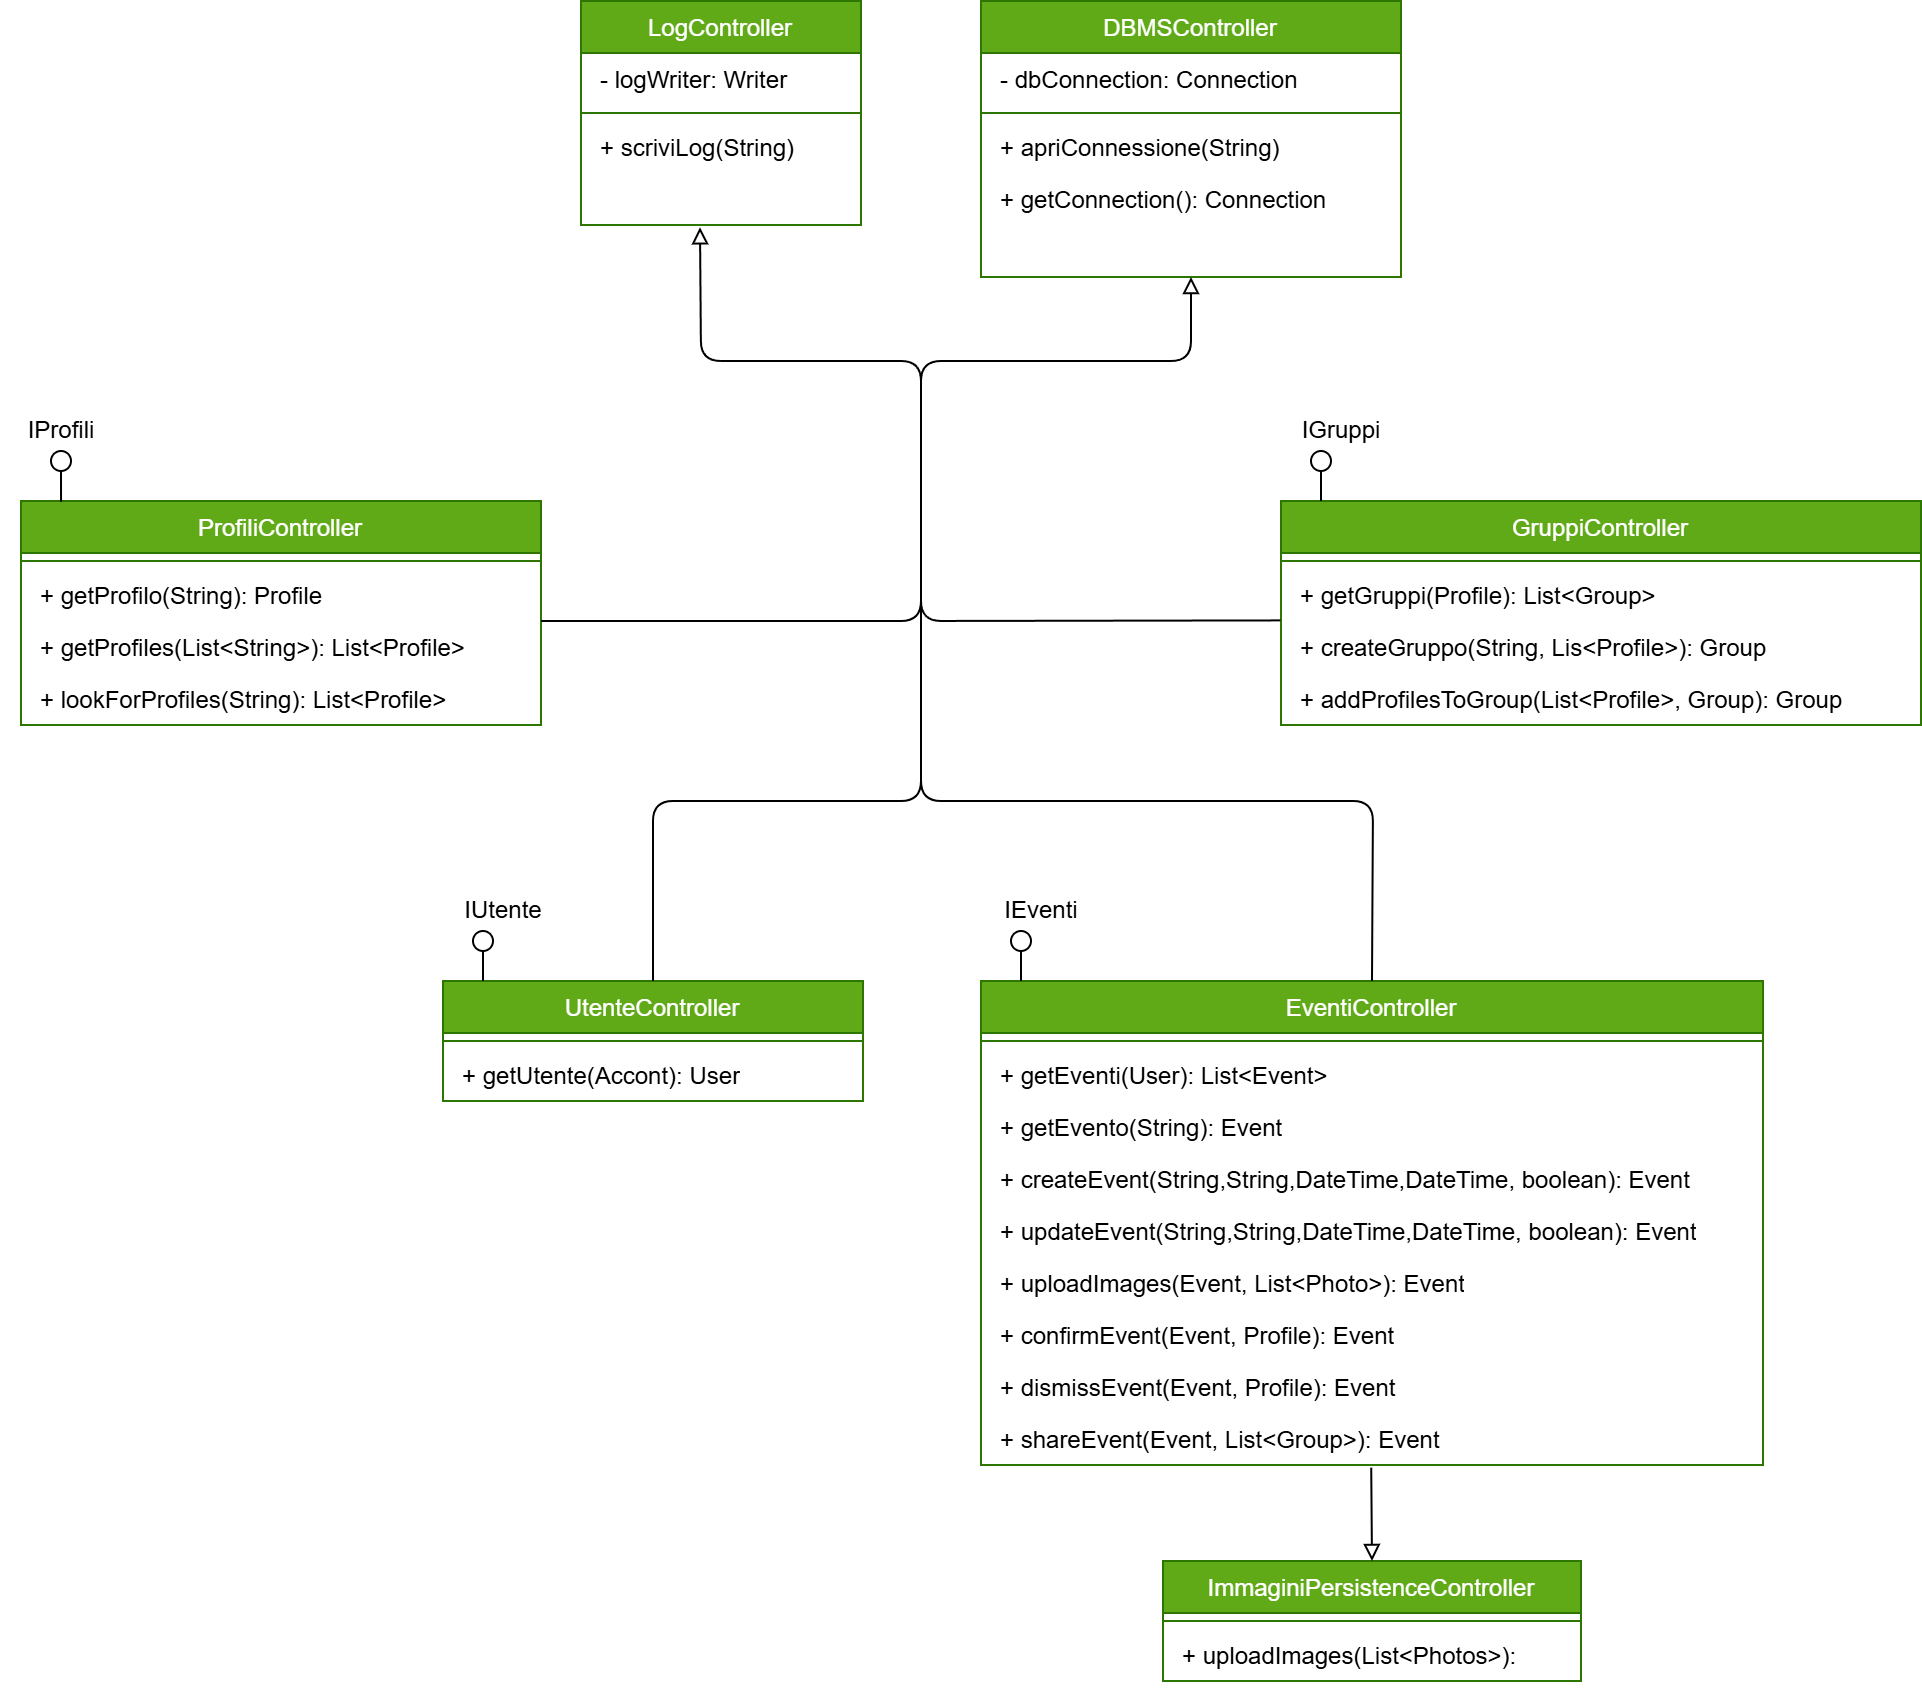
\includegraphics[width=\textwidth]{ProgettoControllerServer.png}
    \end{center}
\end{figure}

\newpage



\textbf{Diagramma di dettaglio: InterfacciaUtente - Eventi}
\begin{figure}[h!]
    \begin{center}
        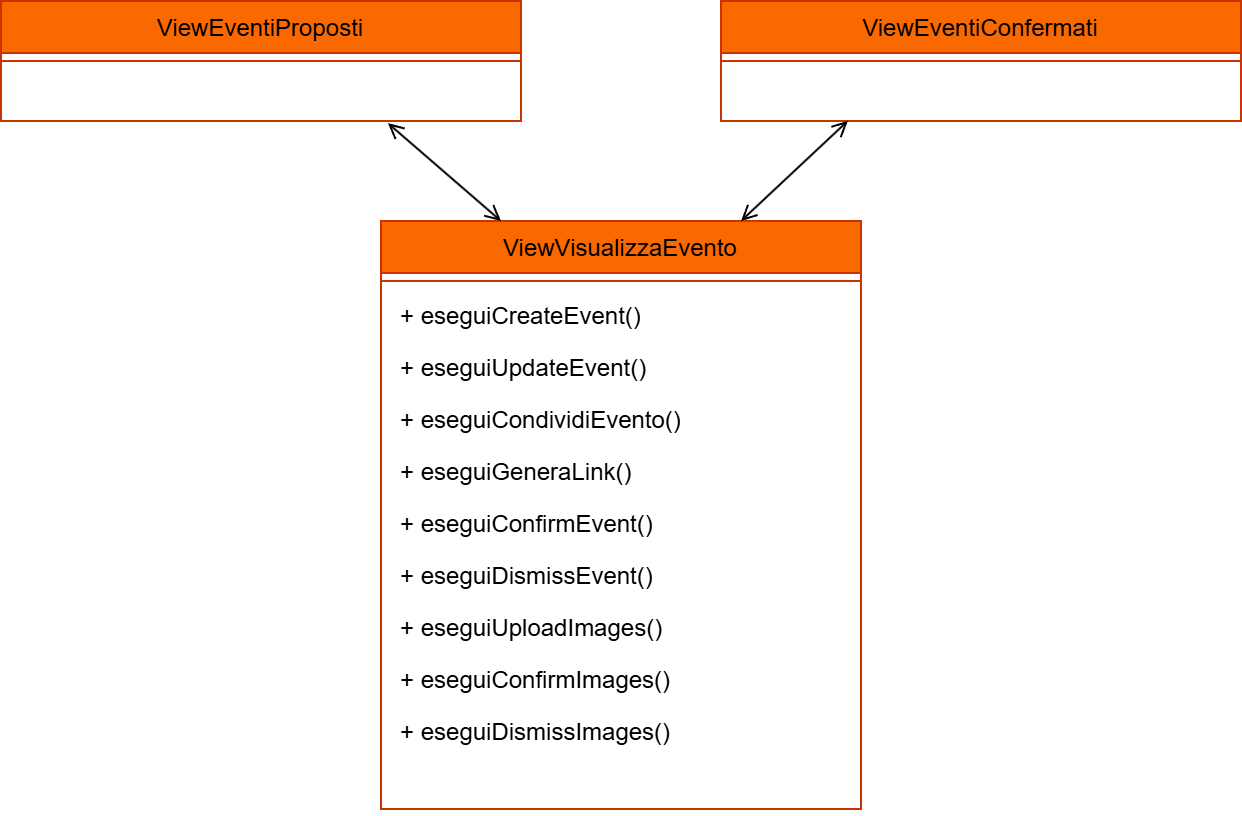
\includegraphics[width=0.9\textwidth]{ProgettoViewEventi.png}
    \end{center}
\end{figure}
\begin{figure}[h!]
    \centering
    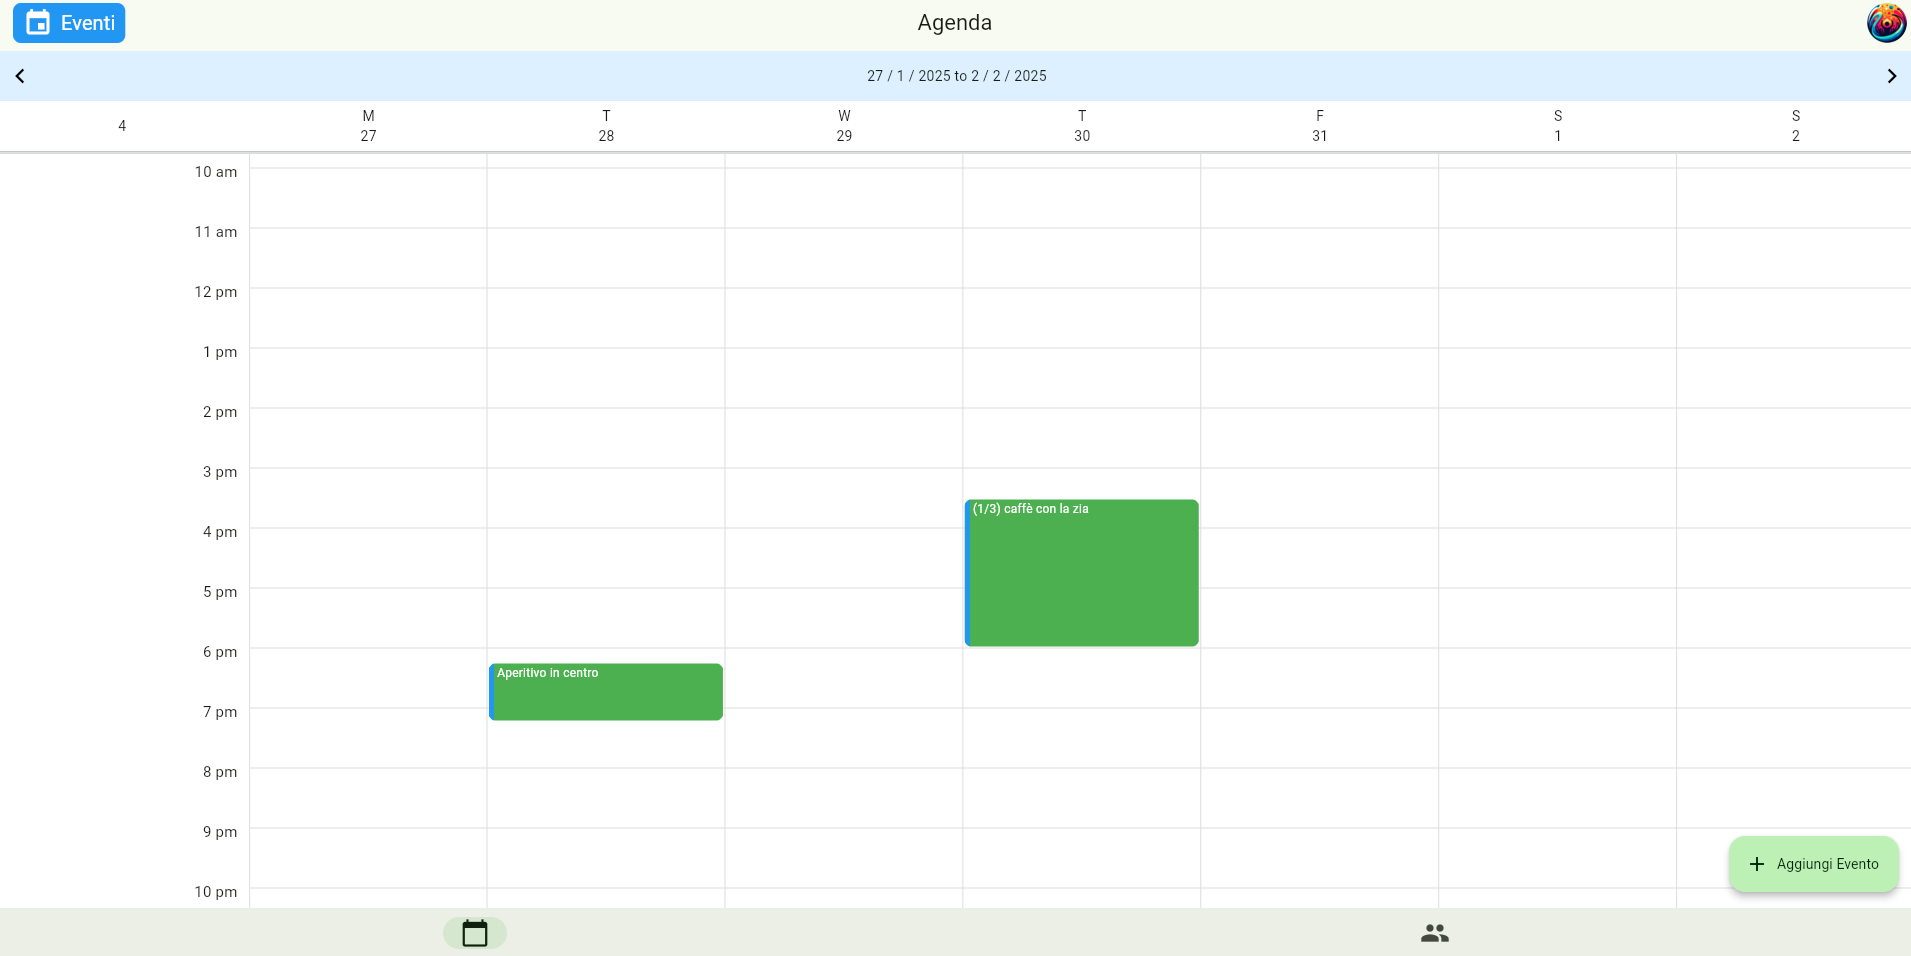
\includegraphics[width=\textwidth]{ProgettoVistaConfermati.png}
    \caption{Eventi confermati}
\end{figure}
\begin{figure}[h!]
    \centering
    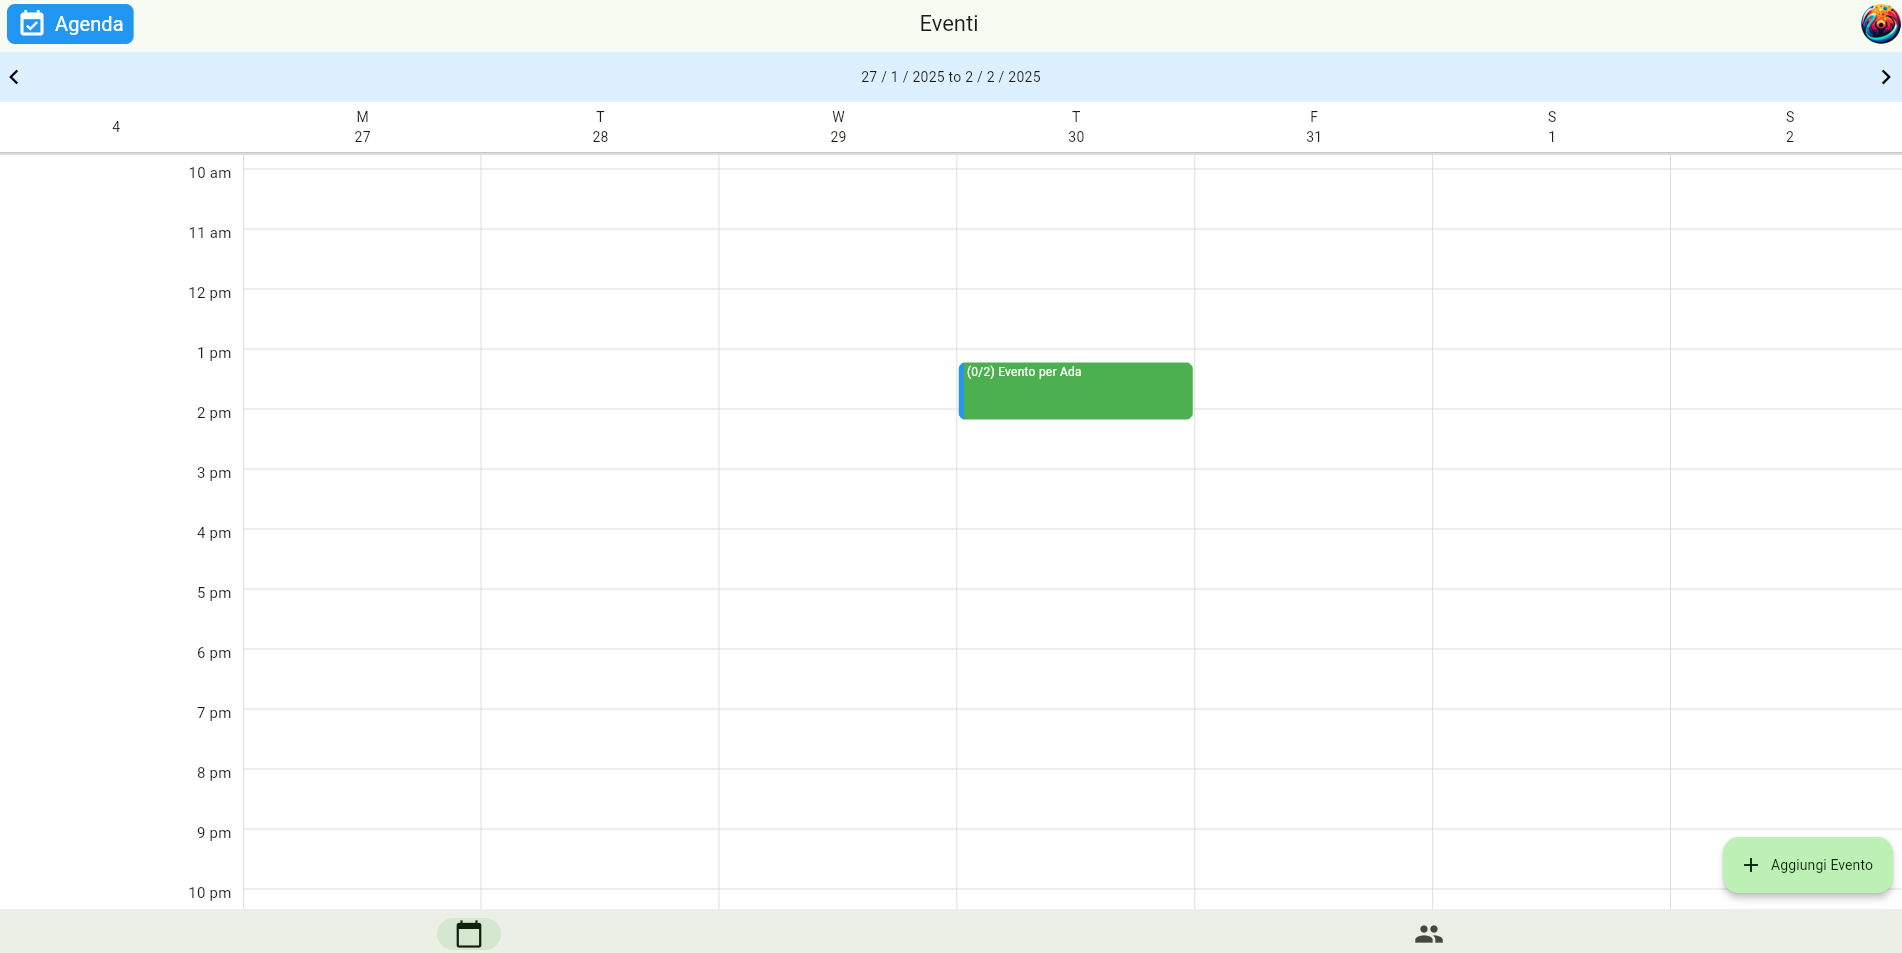
\includegraphics[width=\textwidth]{ProgettoVistaProposti.png}
    \caption{Eventi proposti}
\end{figure}
\begin{figure}[h!]
    \centering
    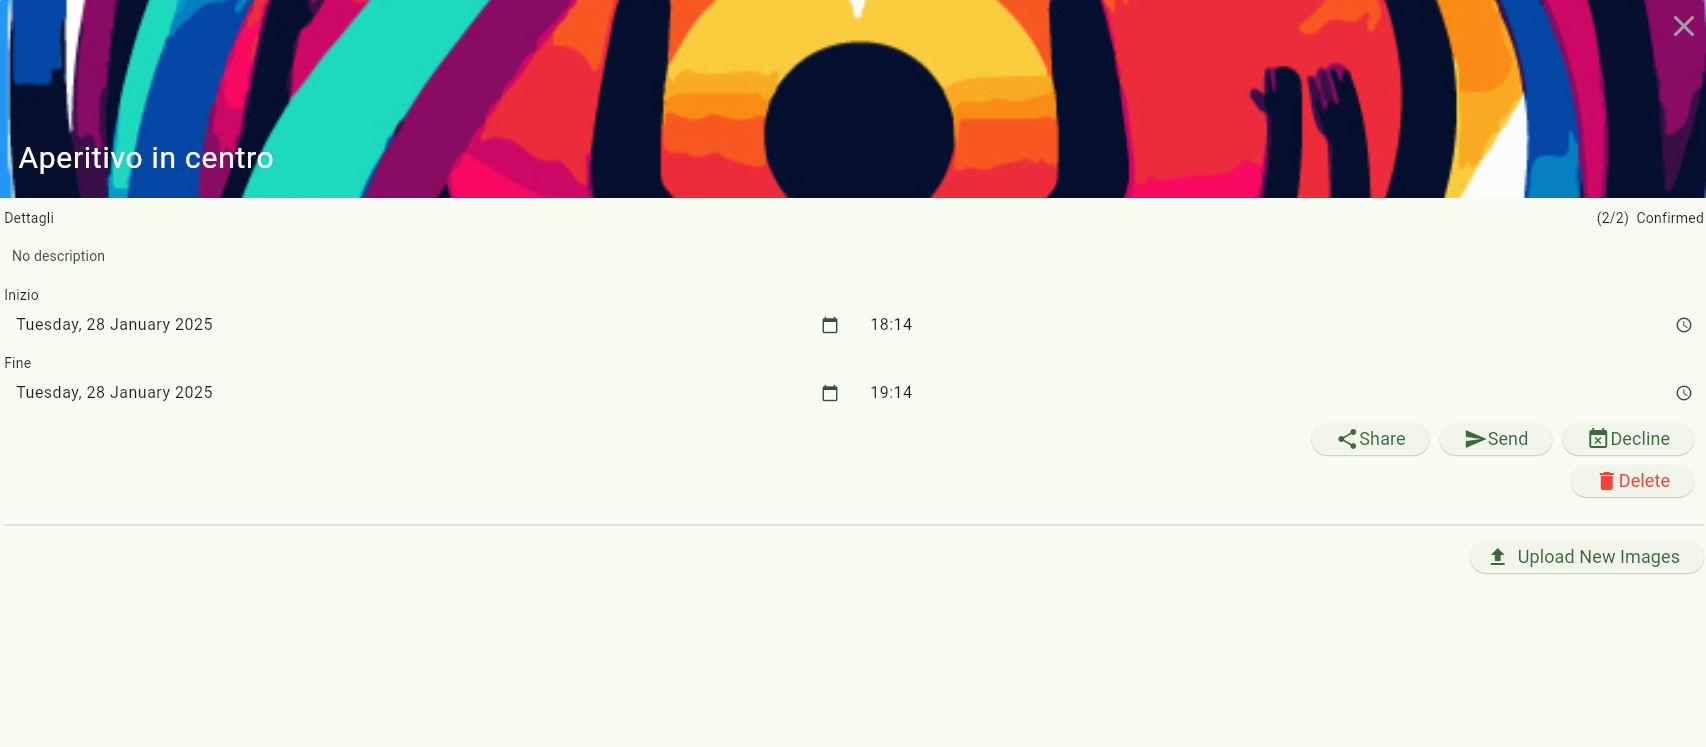
\includegraphics[width=\textwidth]{ProgettoVistaEvento.png}
    \caption{Dettaglio evento}
\end{figure}
\clearpage

\textbf{Diagramma di dettaglio: InterfacciaUtente - Gruppi}
\begin{figure}[h!]
    \begin{center}
        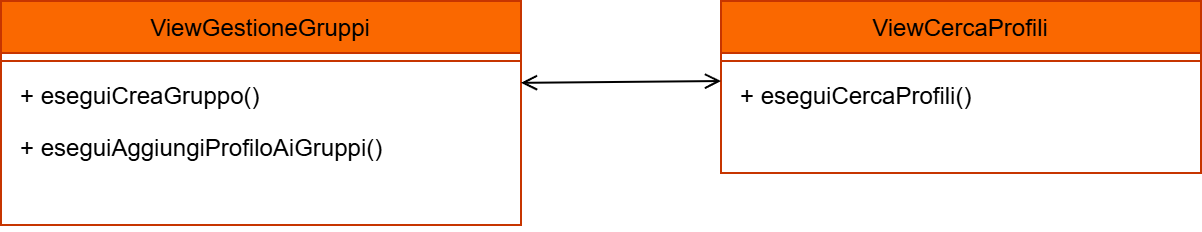
\includegraphics[width=0.9\textwidth]{ProgettoViewGruppi.png}
    \end{center}
\end{figure}
\begin{figure}[h!]
    \centering
    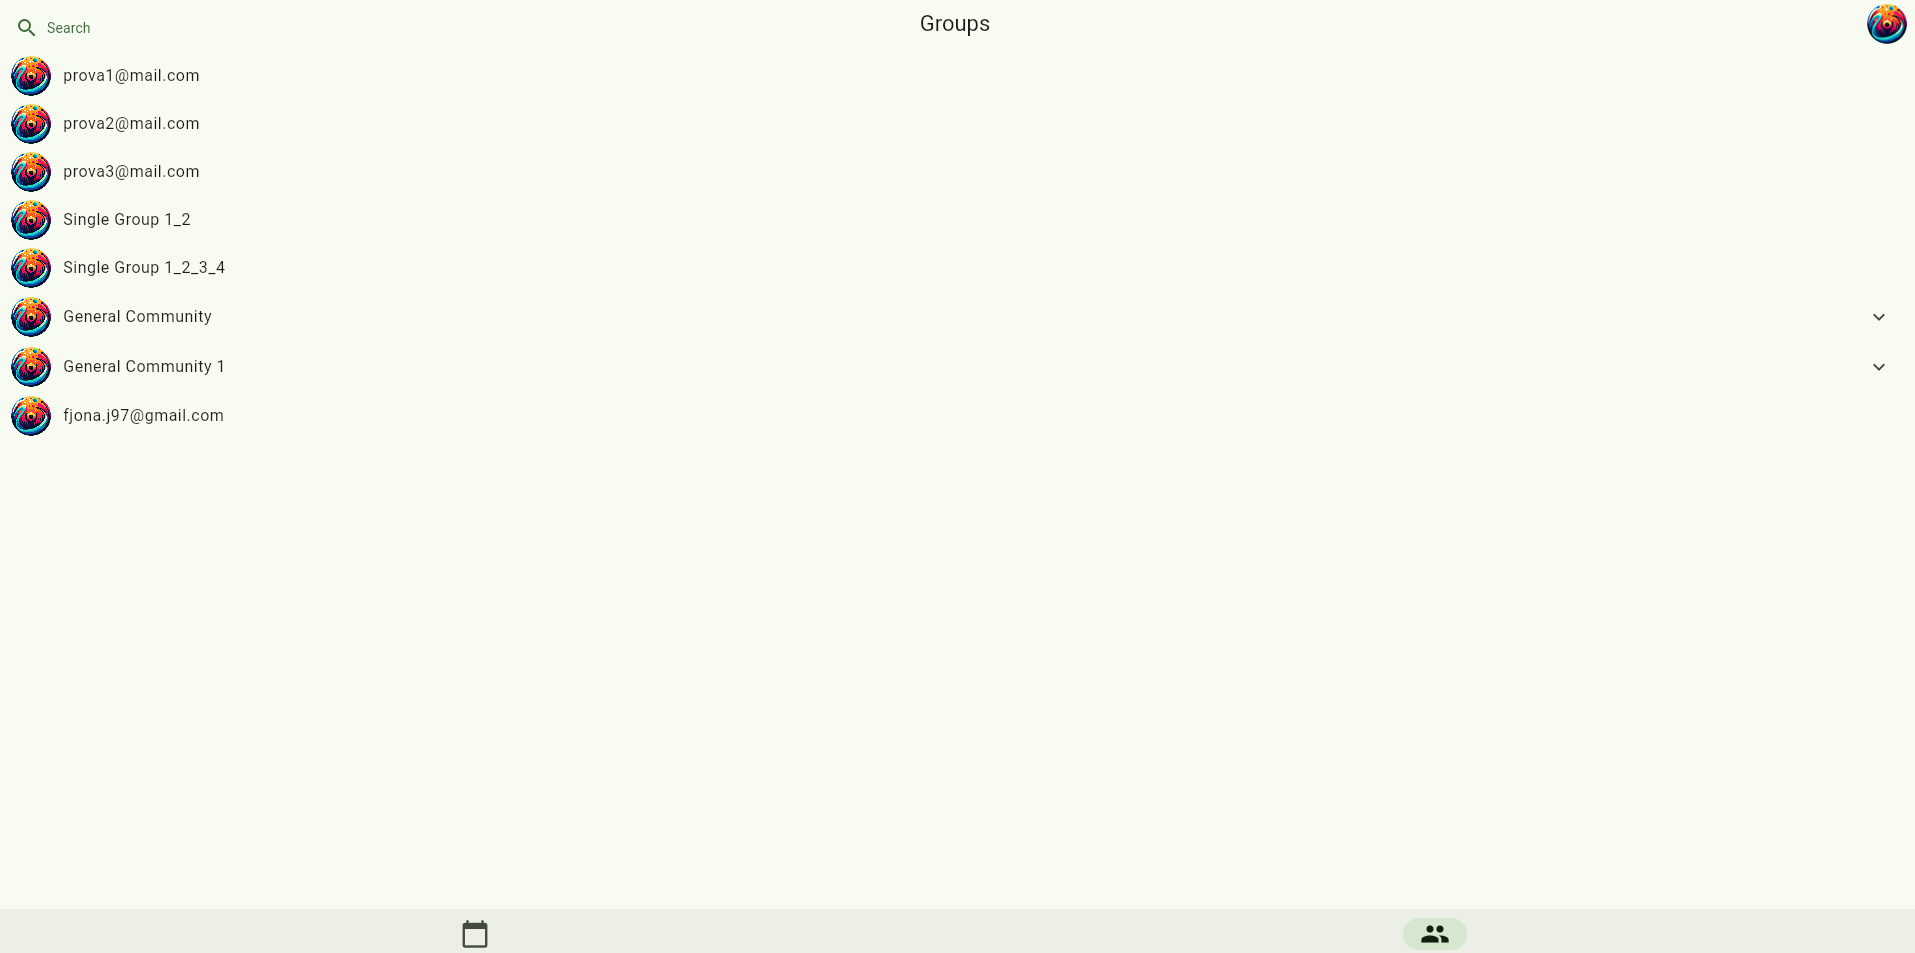
\includegraphics[height=0.28\textheight]{ProgettoVistaGruppi.png}
    \caption{Gruppi}
\end{figure}
\begin{figure}[h!]
    \centering
    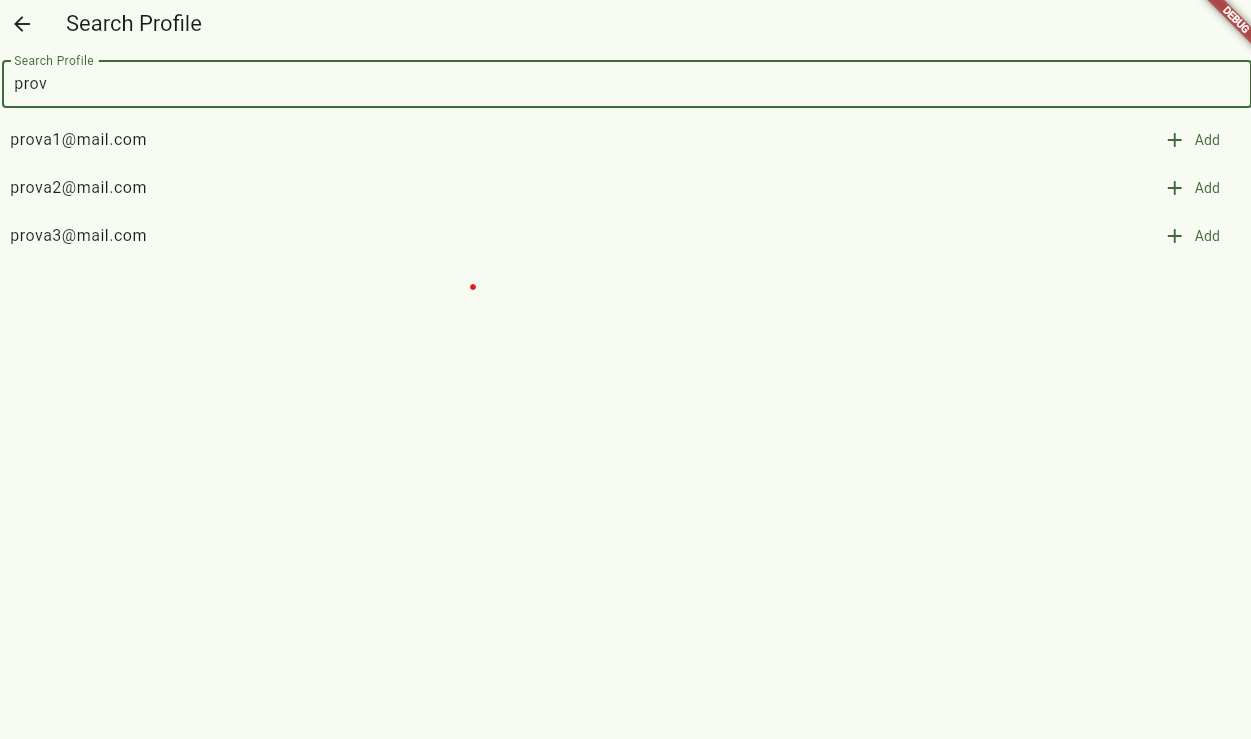
\includegraphics[height=0.33\textheight]{ProgettoVistaCercaProfili.png}
    \caption{Cerca profili}
\end{figure}
\clearpage

\textbf{Diagramma di dettaglio: InterfacciaUtente - Profili}
\begin{figure}[h!]
    \begin{center}
        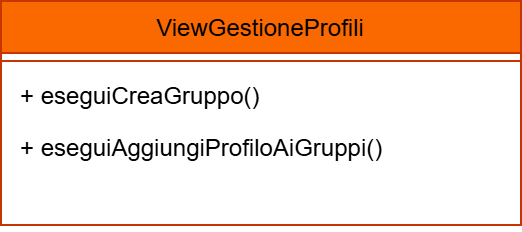
\includegraphics[width=0.6\textwidth]{ProgettoViewProfili.png}
    \end{center}
\end{figure}

\begin{figure}[h!]
    \centering
    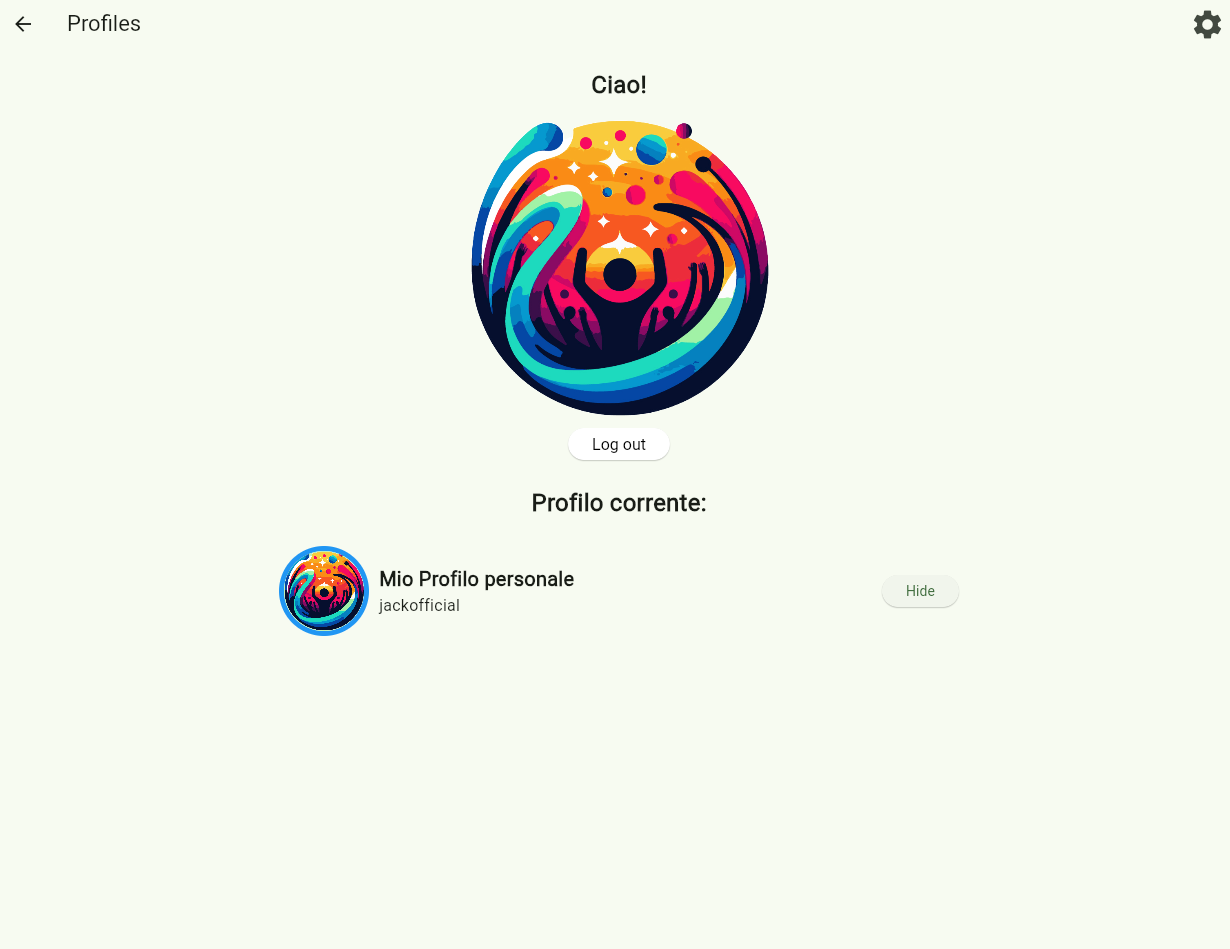
\includegraphics[width=\textwidth]{ProgettoVistaProfili.png}
    \caption{Profili collegati}
\end{figure}

\newpage

\textbf{Diagramma di dettaglio: InterfacciaGestioneAccesso}

\begin{figure}[h!]
    \begin{center}
        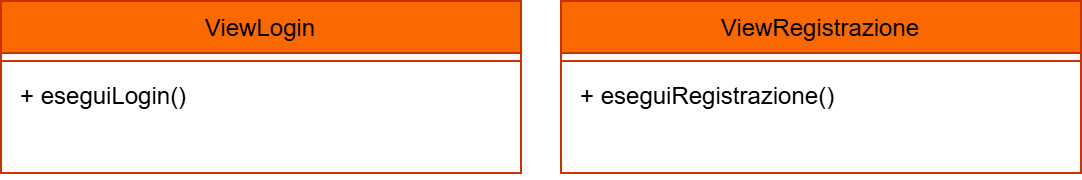
\includegraphics[width=0.9\textwidth]{ProgettoViewGestioneAccesso.png}
    \end{center}
\end{figure}

\begin{figure}[h!]
    \centering
    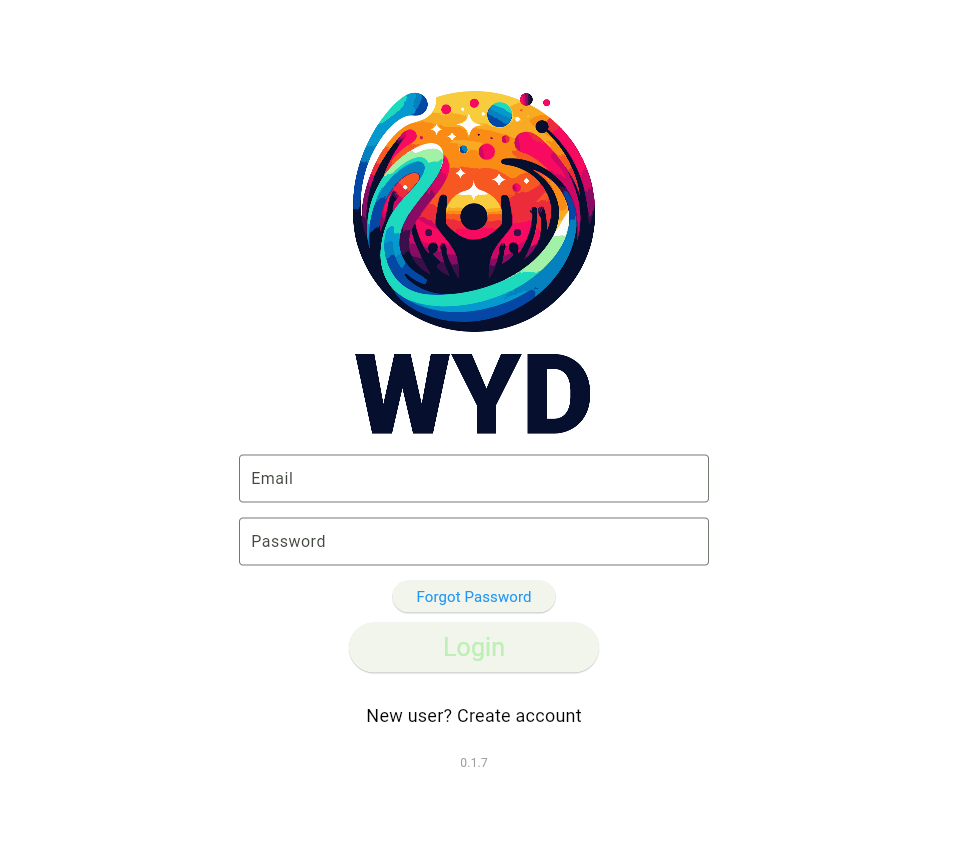
\includegraphics[width=\textwidth]{ProgettoVistaLogin.png}
    \caption{Login}
\end{figure}
\begin{figure}[h!]
    \centering
    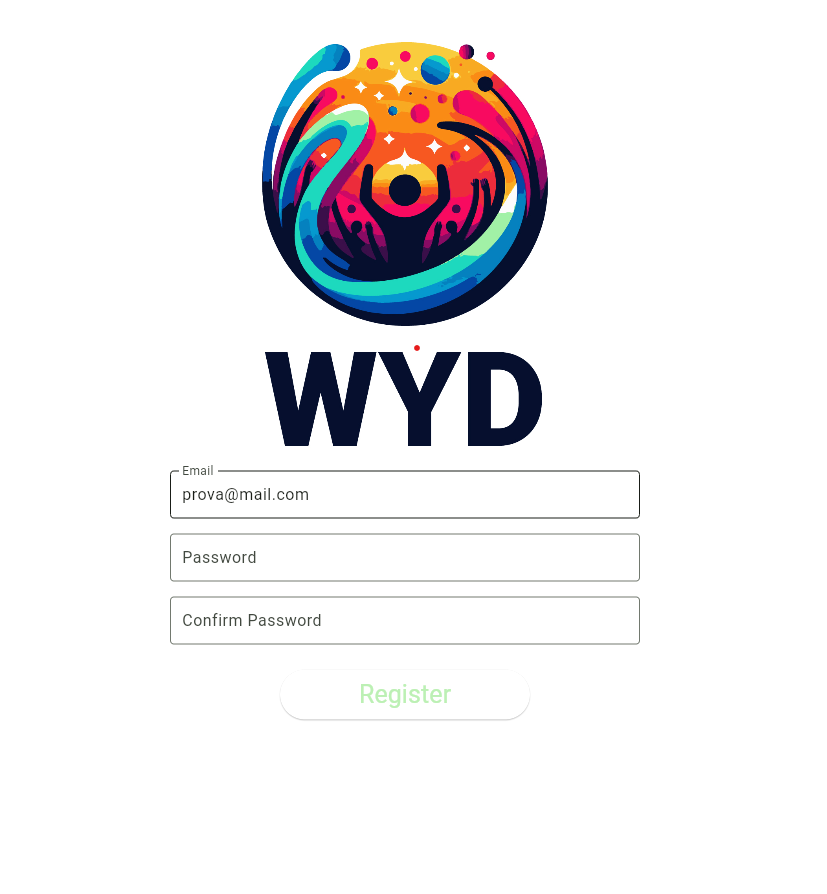
\includegraphics[width=\textwidth]{ProgettoVistaRegistrazione.png}
    \caption{Registrazione}
\end{figure}

\clearpage



\subsubsection{Interazione}


Si riportano di seguito i vari diagrammi di sequenza, aggiornati rispetto a quelli visti in fase di analisi.\\
\vspace{3em}

\textbf{Diagramma di Sequenza: Registrazione - Client}
\begin{figure}[h!]
    \centering
    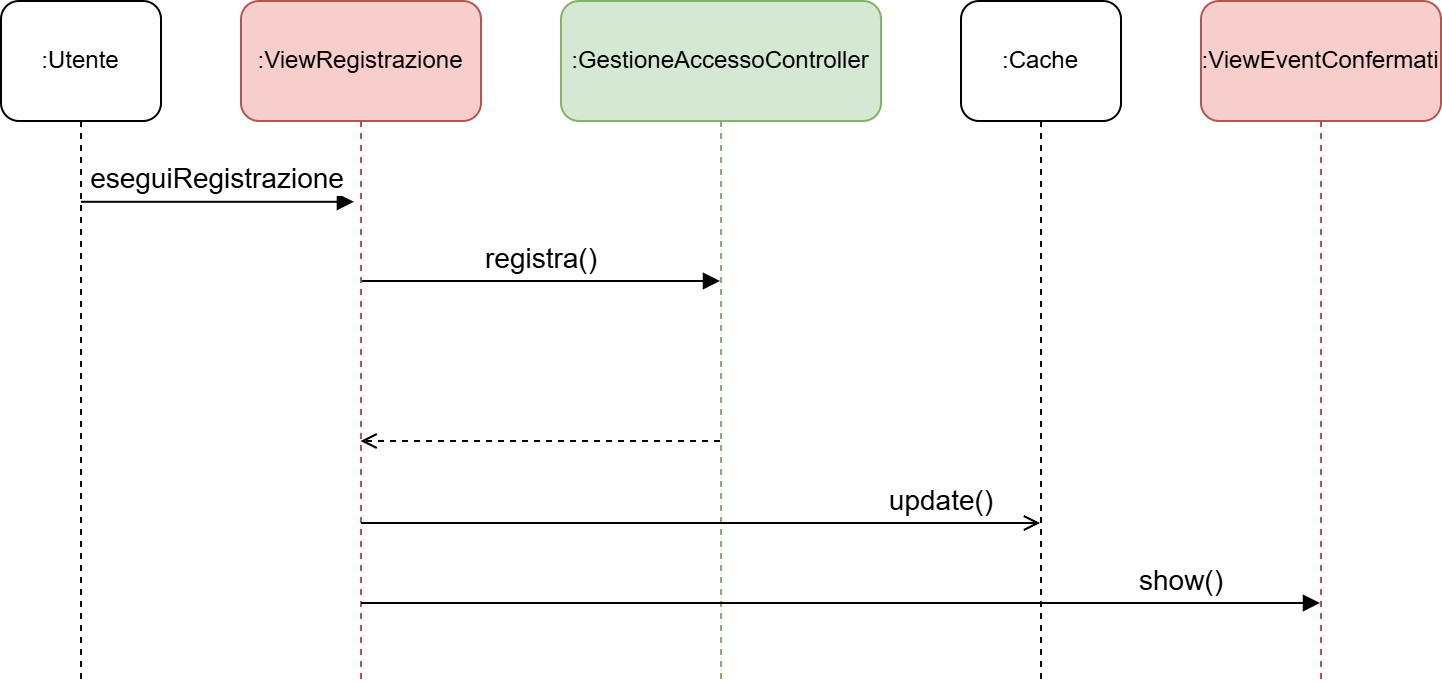
\includegraphics[width=\textwidth]{PIRegistrazione1.png}
\end{figure}

\textbf{Diagramma di Sequenza: Registrazione - Server}
\begin{figure}[h!]
    \centering
    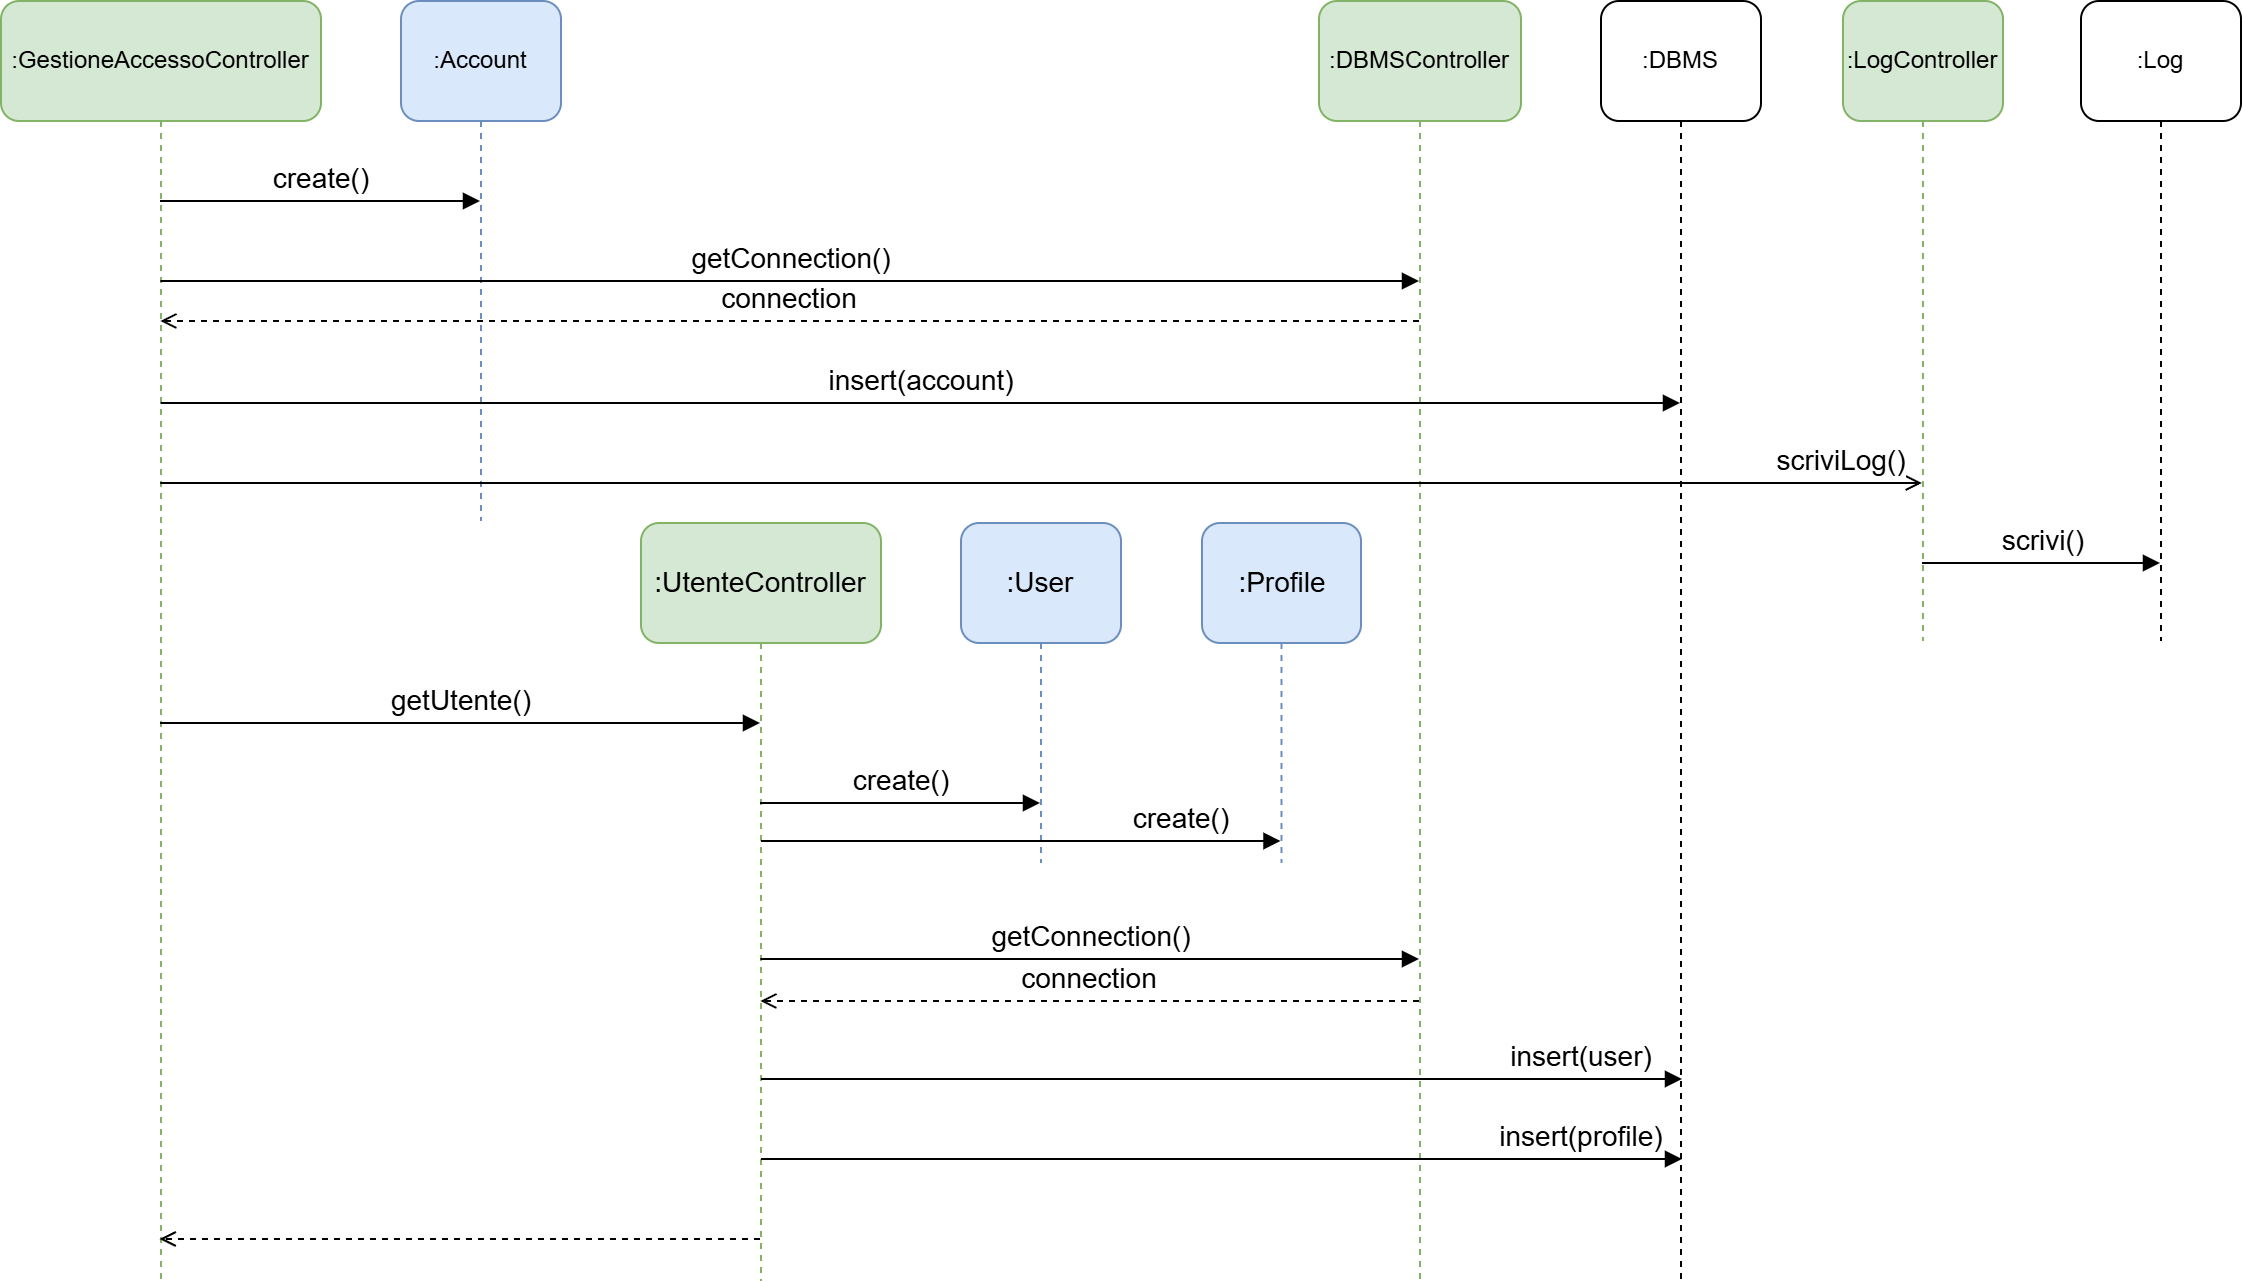
\includegraphics[width=\textwidth]{PIRegistrazione2.png}
\end{figure}
\clearpage
\textbf{Diagramma di Sequenza: Visualizza Eventi Confermati}
\begin{figure}[h!]
    \centering
    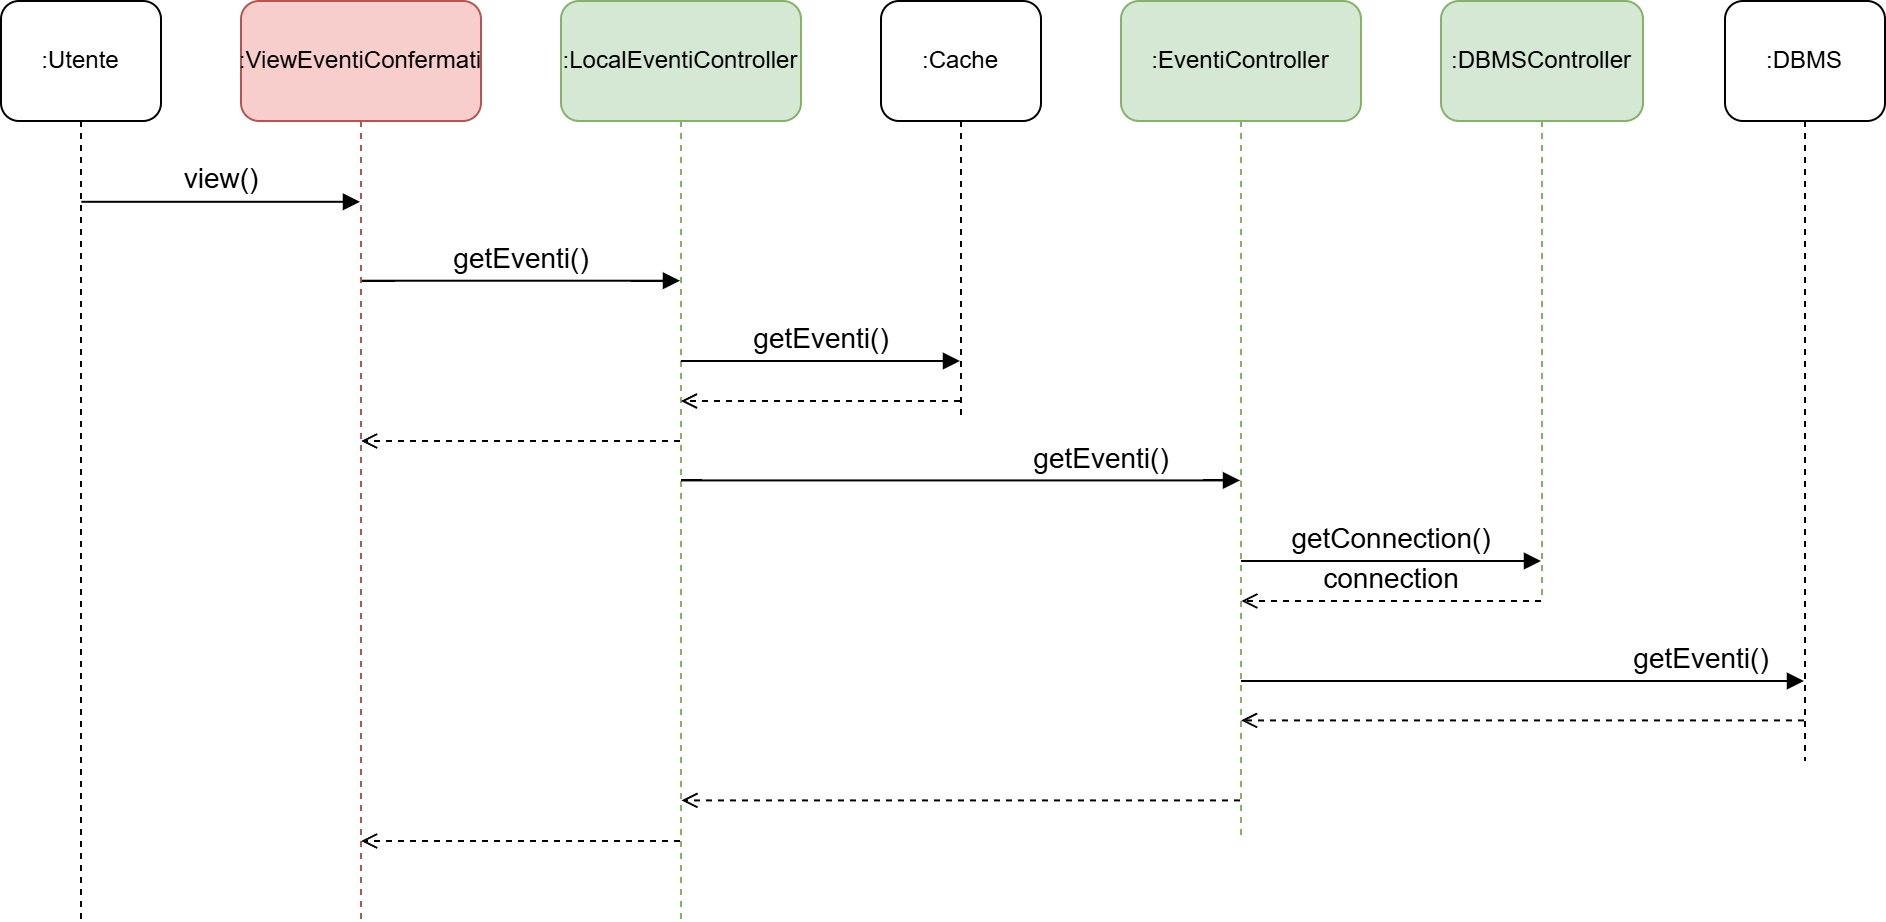
\includegraphics[width=\textwidth]{PIVisualizzaEventiConfermati.png}
\end{figure}\\
\textbf{Diagramma di Sequenza: Visualizza Evento}
\begin{figure}[h!]
    \centering
    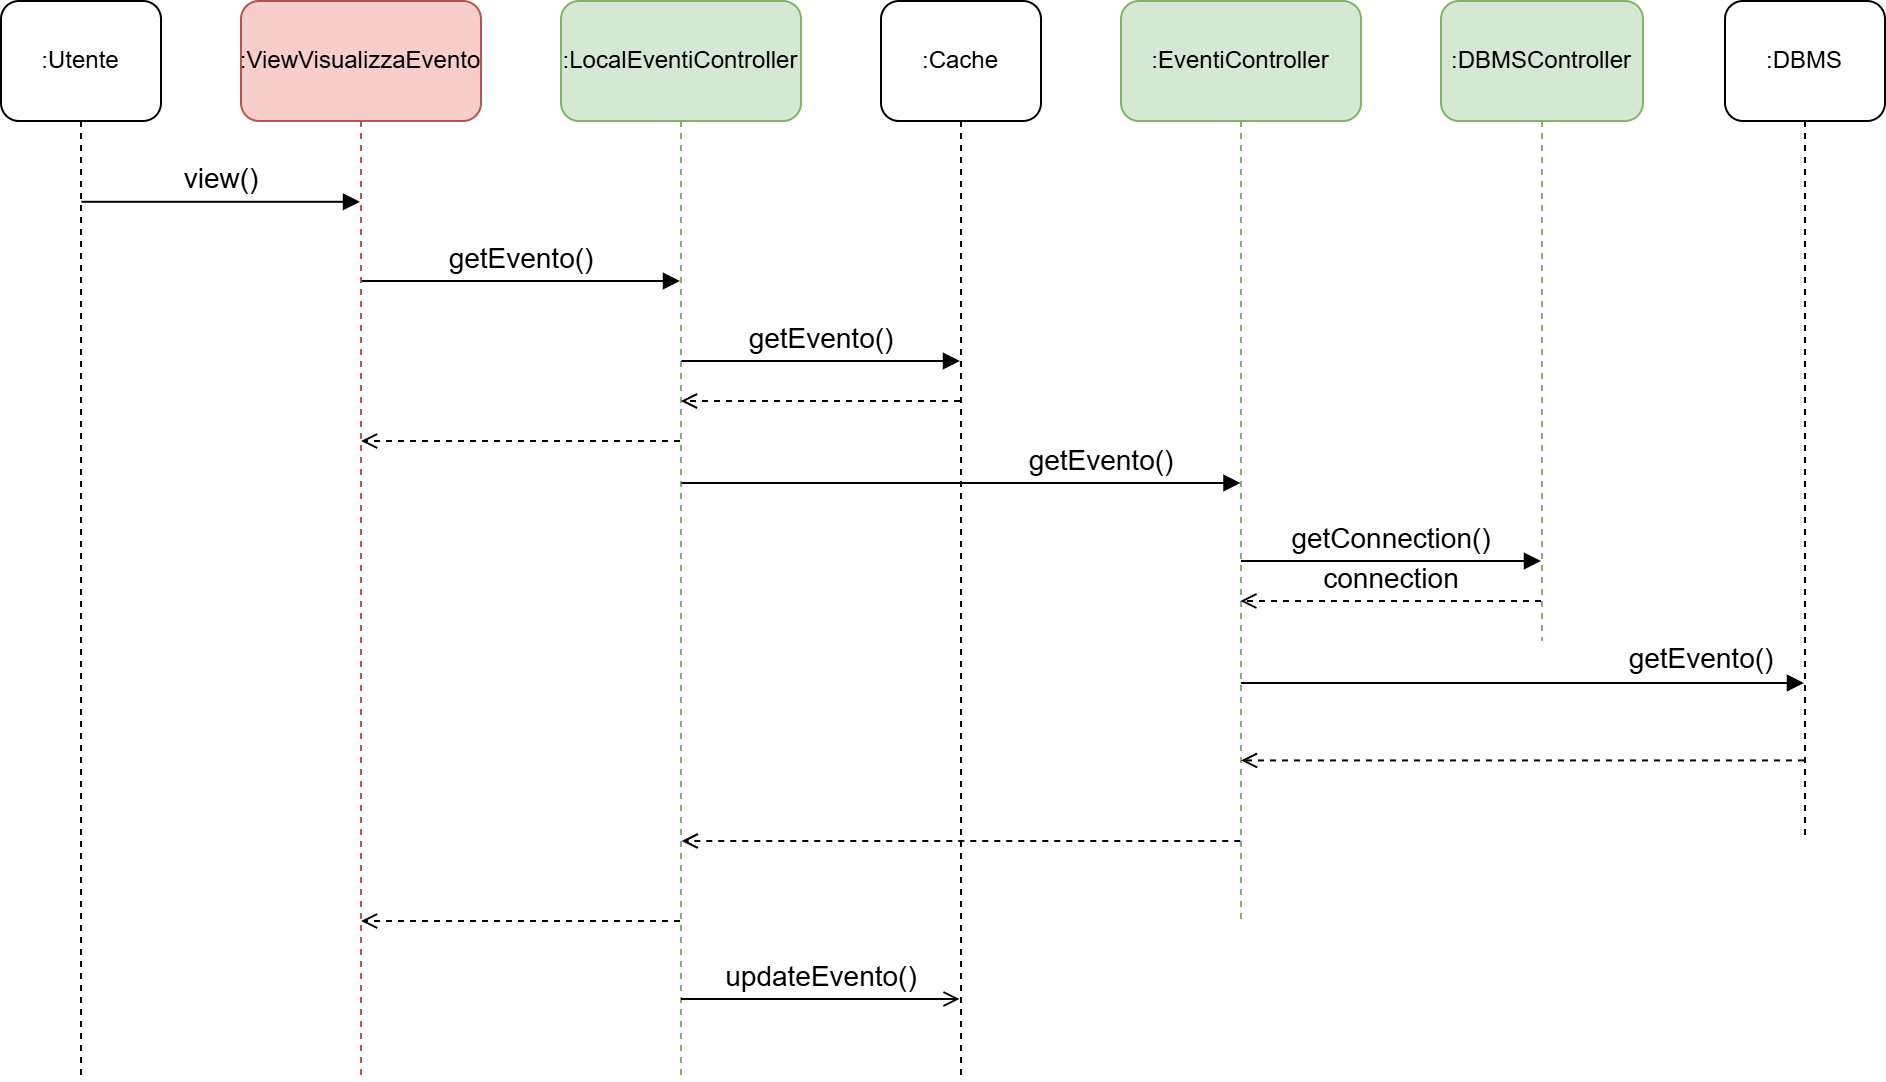
\includegraphics[width=\textwidth]{PIVisualizzaEvento.png}
\end{figure}
\clearpage
\textbf{Diagramma di Sequenza: Crea Evento}
\begin{figure}[h!]
    \centering
    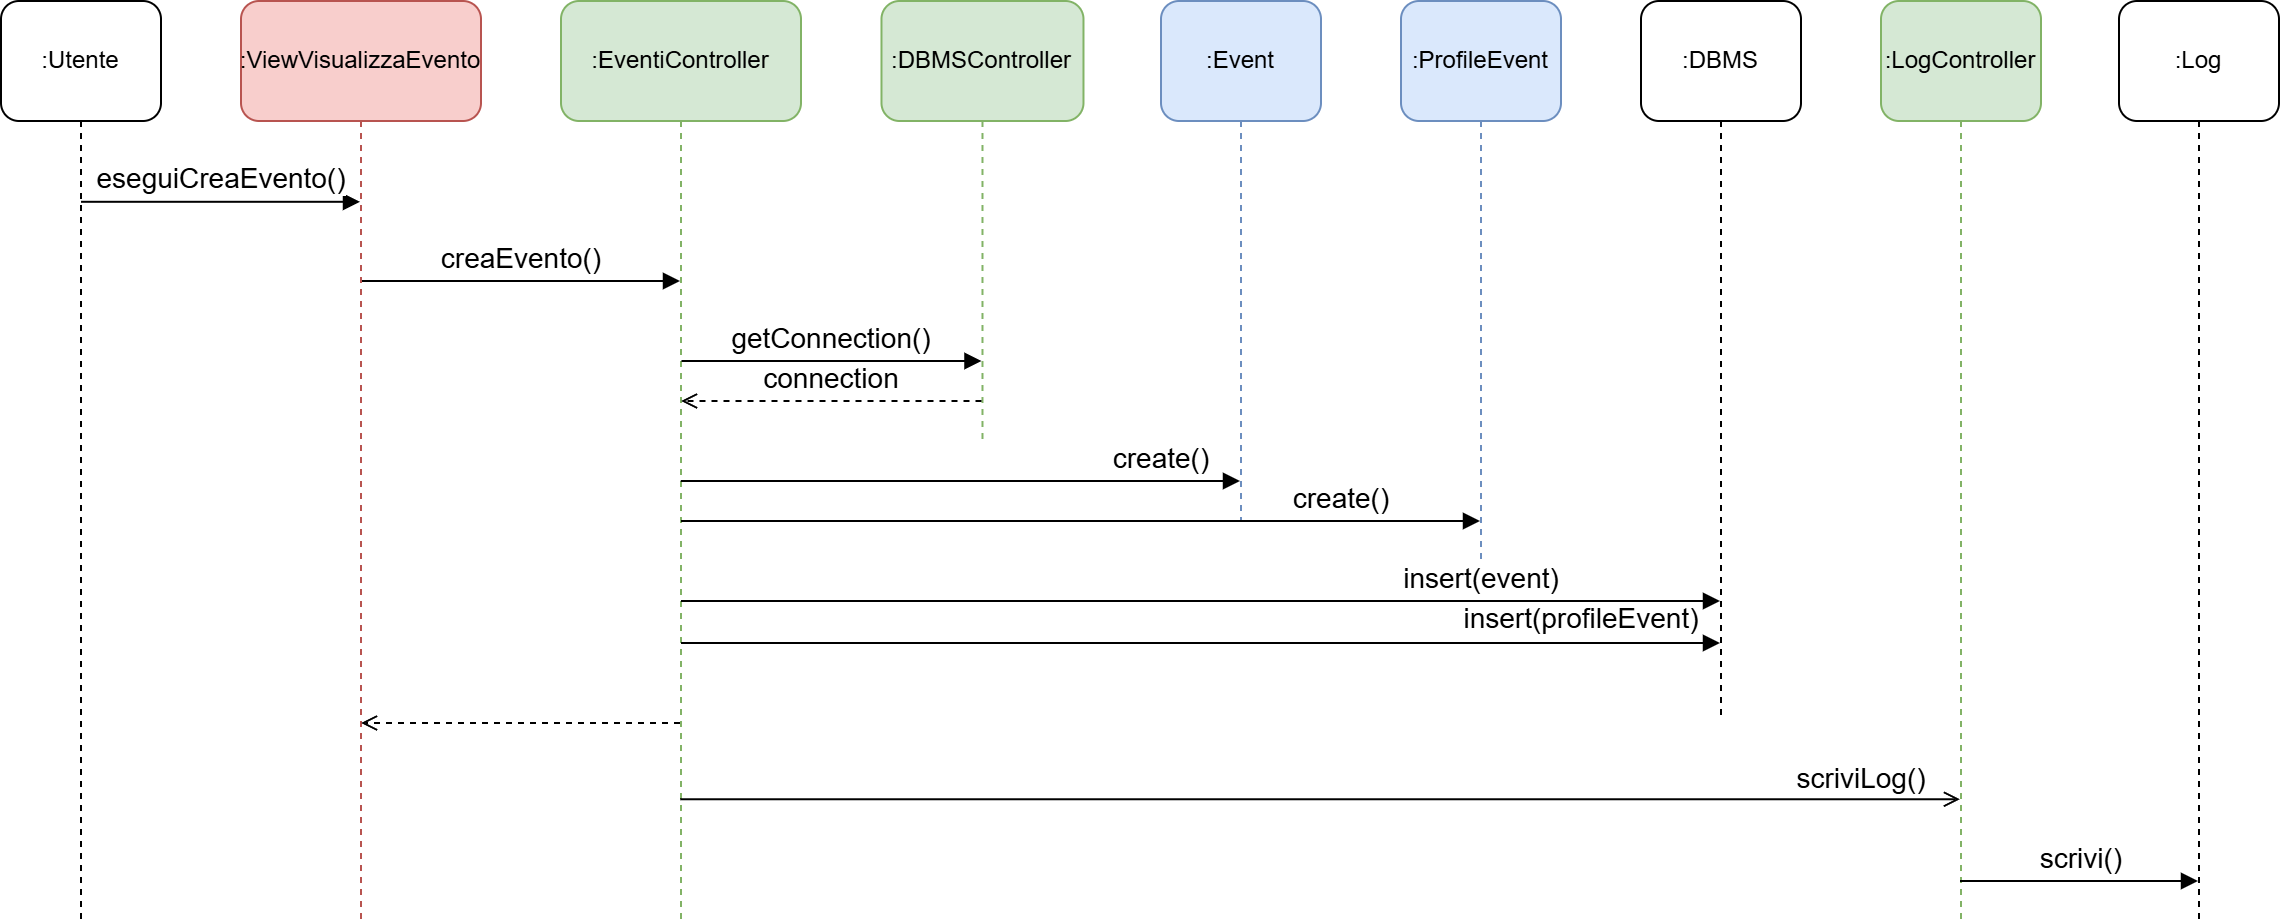
\includegraphics[width=\textwidth]{PICreaEvento.png}
\end{figure}\\
\textbf{Diagramma di Sequenza: Modifica Evento}
\begin{figure}[h!]
    \centering
    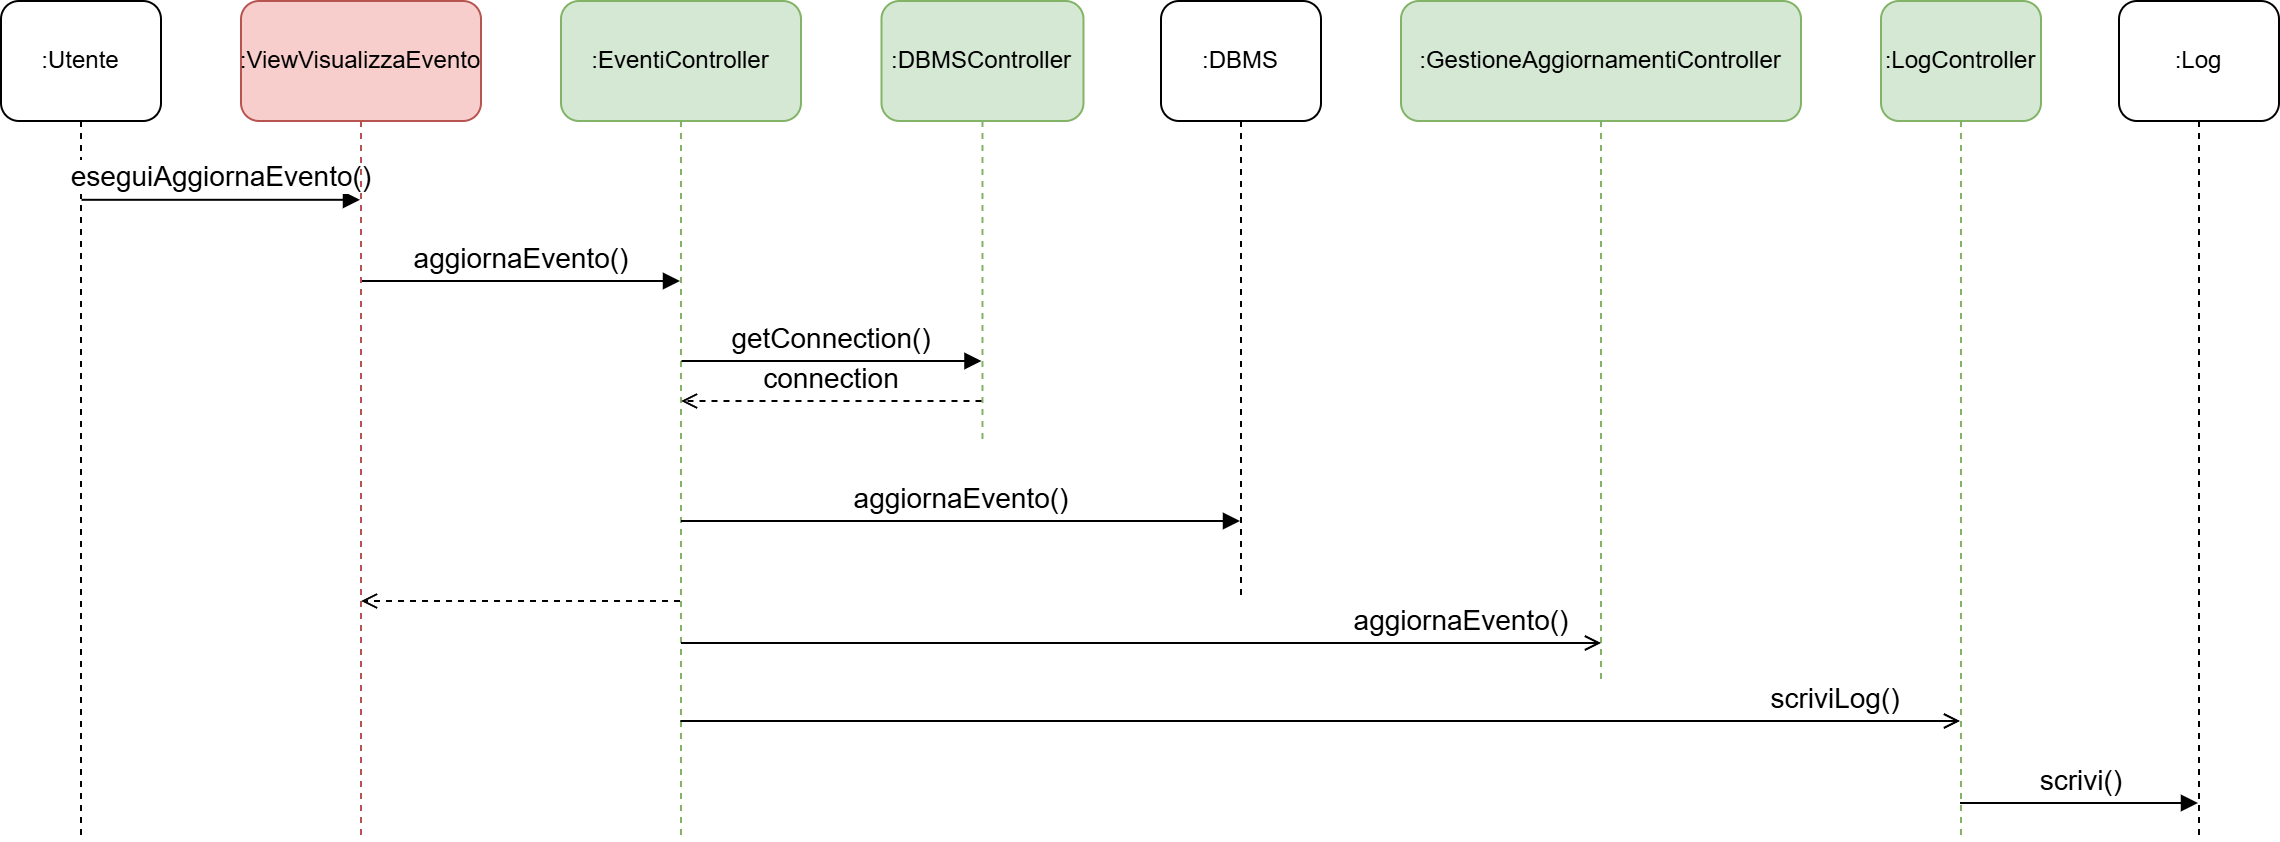
\includegraphics[width=\textwidth]{PIModificaEvento.png}
\end{figure}\\
\textbf{Diagramma di Sequenza: Aggiorna Evento}
\begin{figure}[h!]
    \centering
    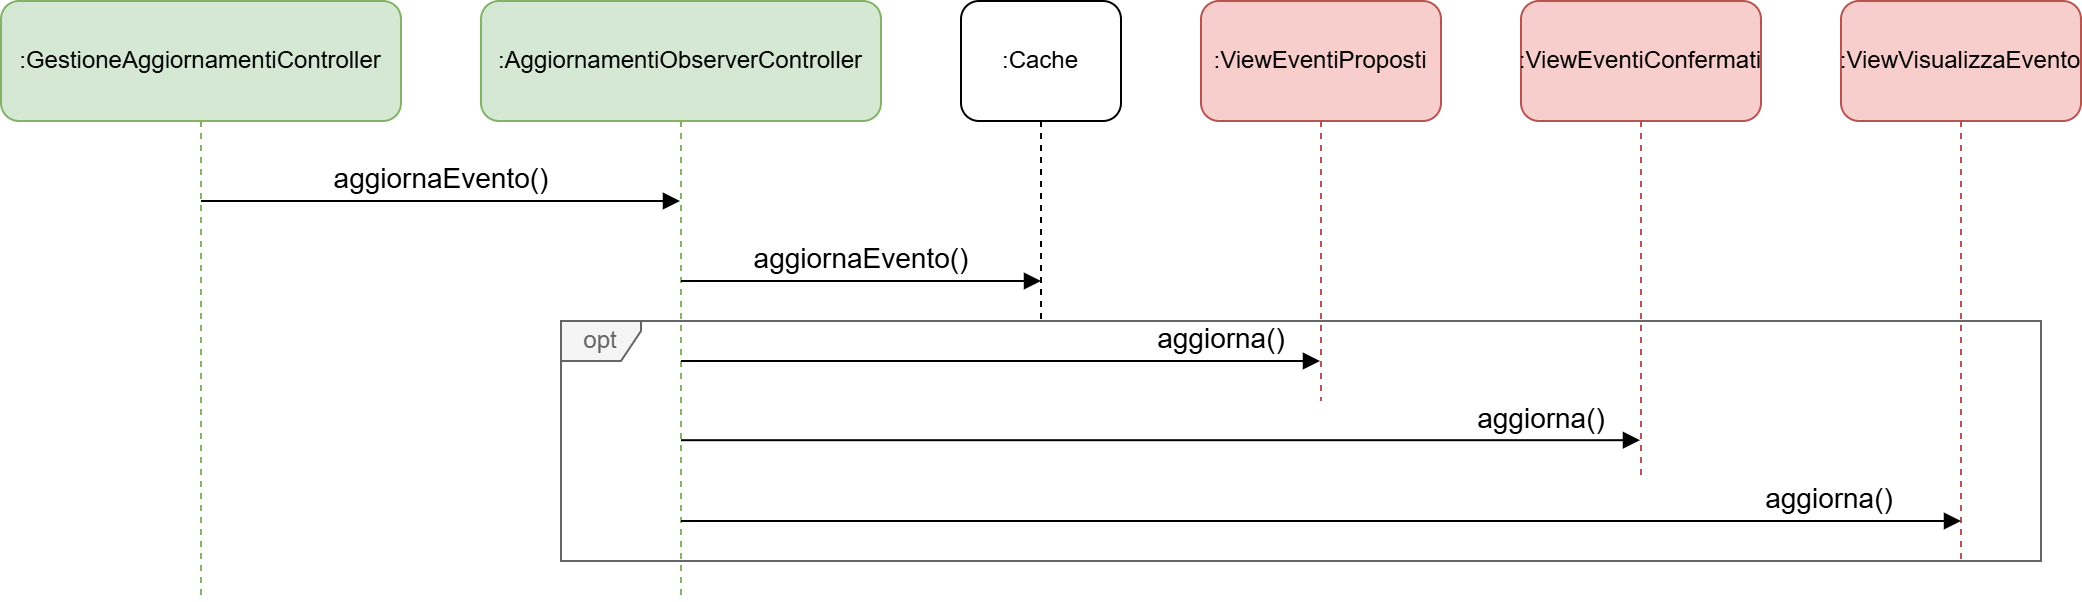
\includegraphics[width=\textwidth]{PIAggiornaEvento.png}
\end{figure}
\clearpage
\textbf{Diagramma di Sequenza: Conferma Evento}
\begin{figure}[h!]
    \centering
    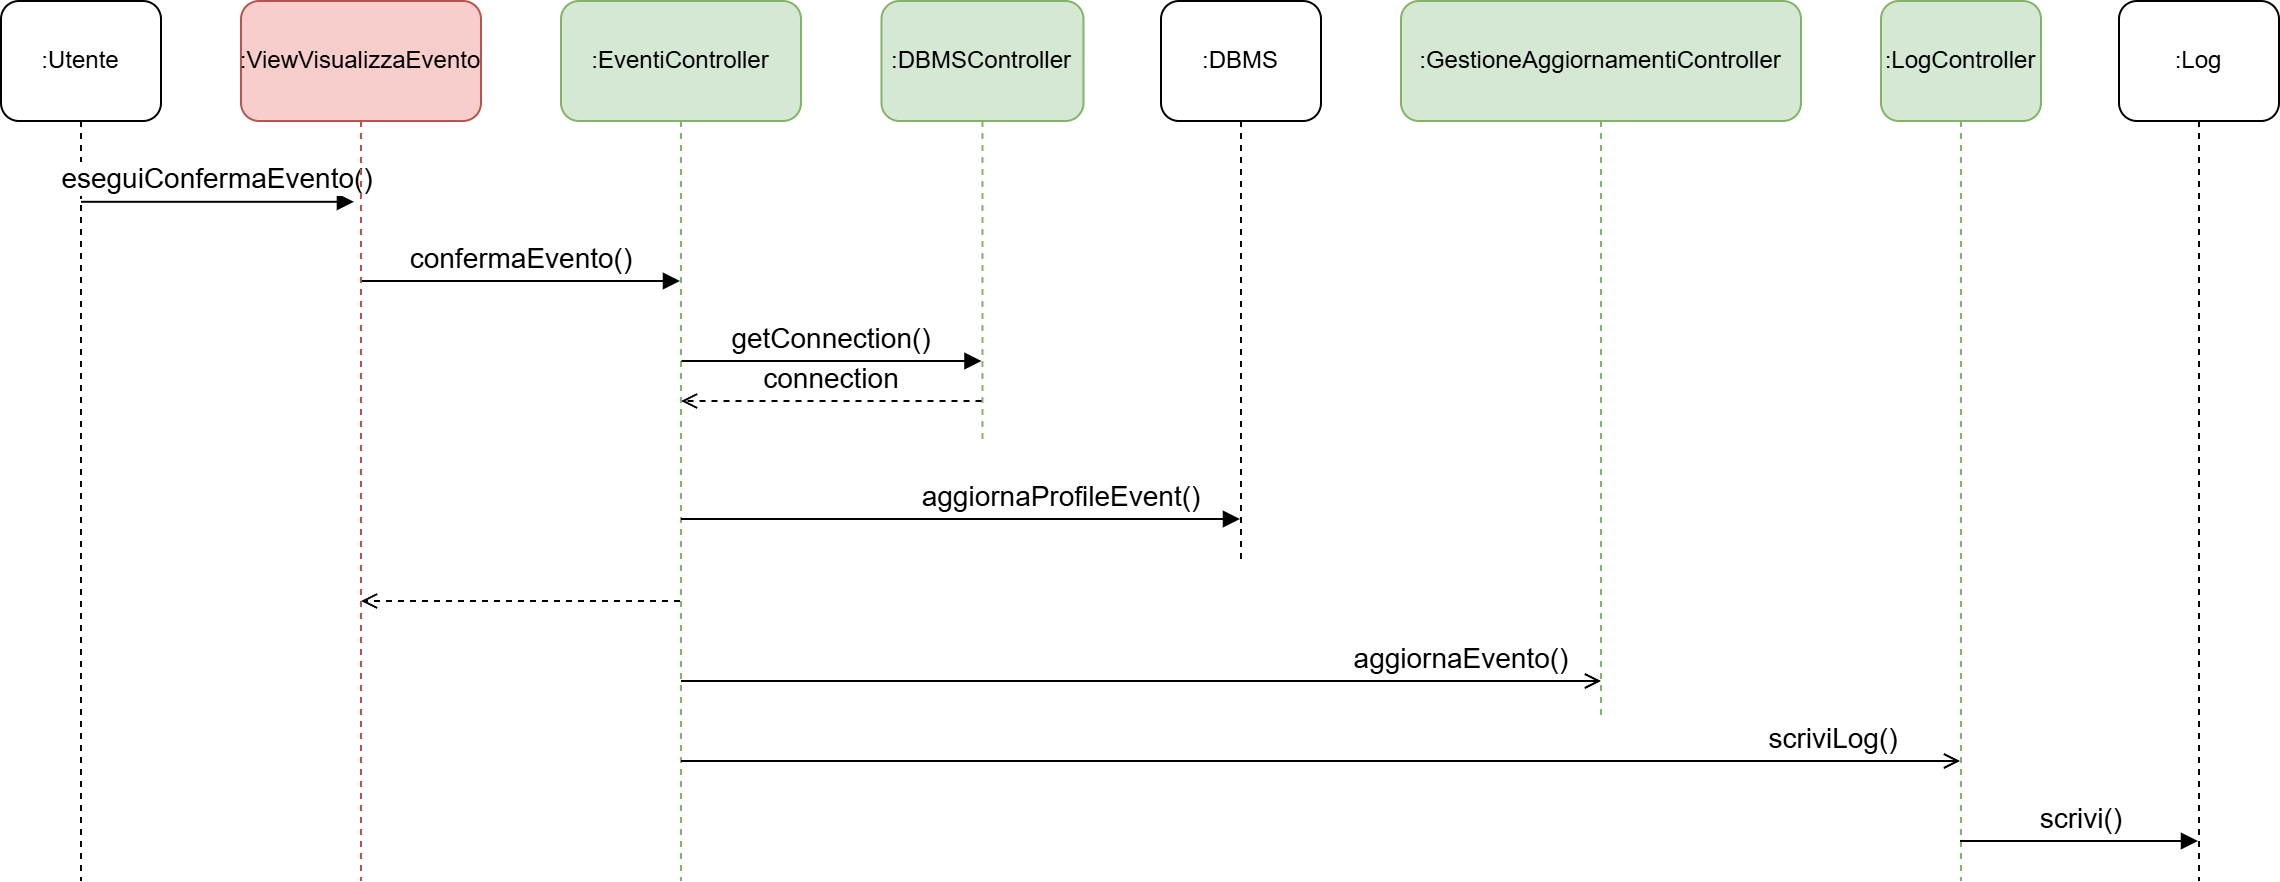
\includegraphics[width=\textwidth]{PIConfermaEvento.png}
\end{figure}

\textbf{Diagramma di Sequenza: Recupera Immagini - Client}
\begin{figure}[h!]
    \centering
    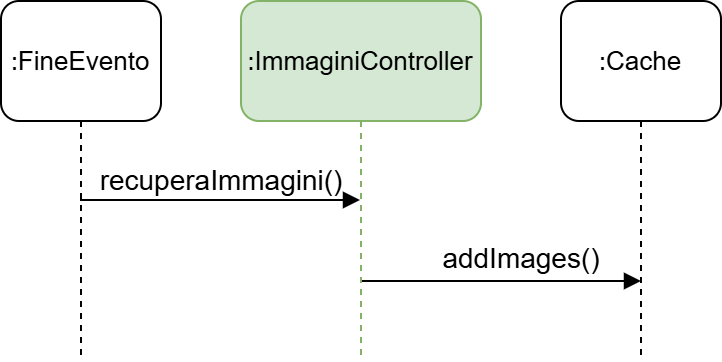
\includegraphics[width=0.8\textwidth]{PIRecuperaImmagini.png}
\end{figure}
\clearpage

\textbf{Diagramma di Sequenza: Conferma Immagini - Client}
\begin{figure}[h!]
    \centering
    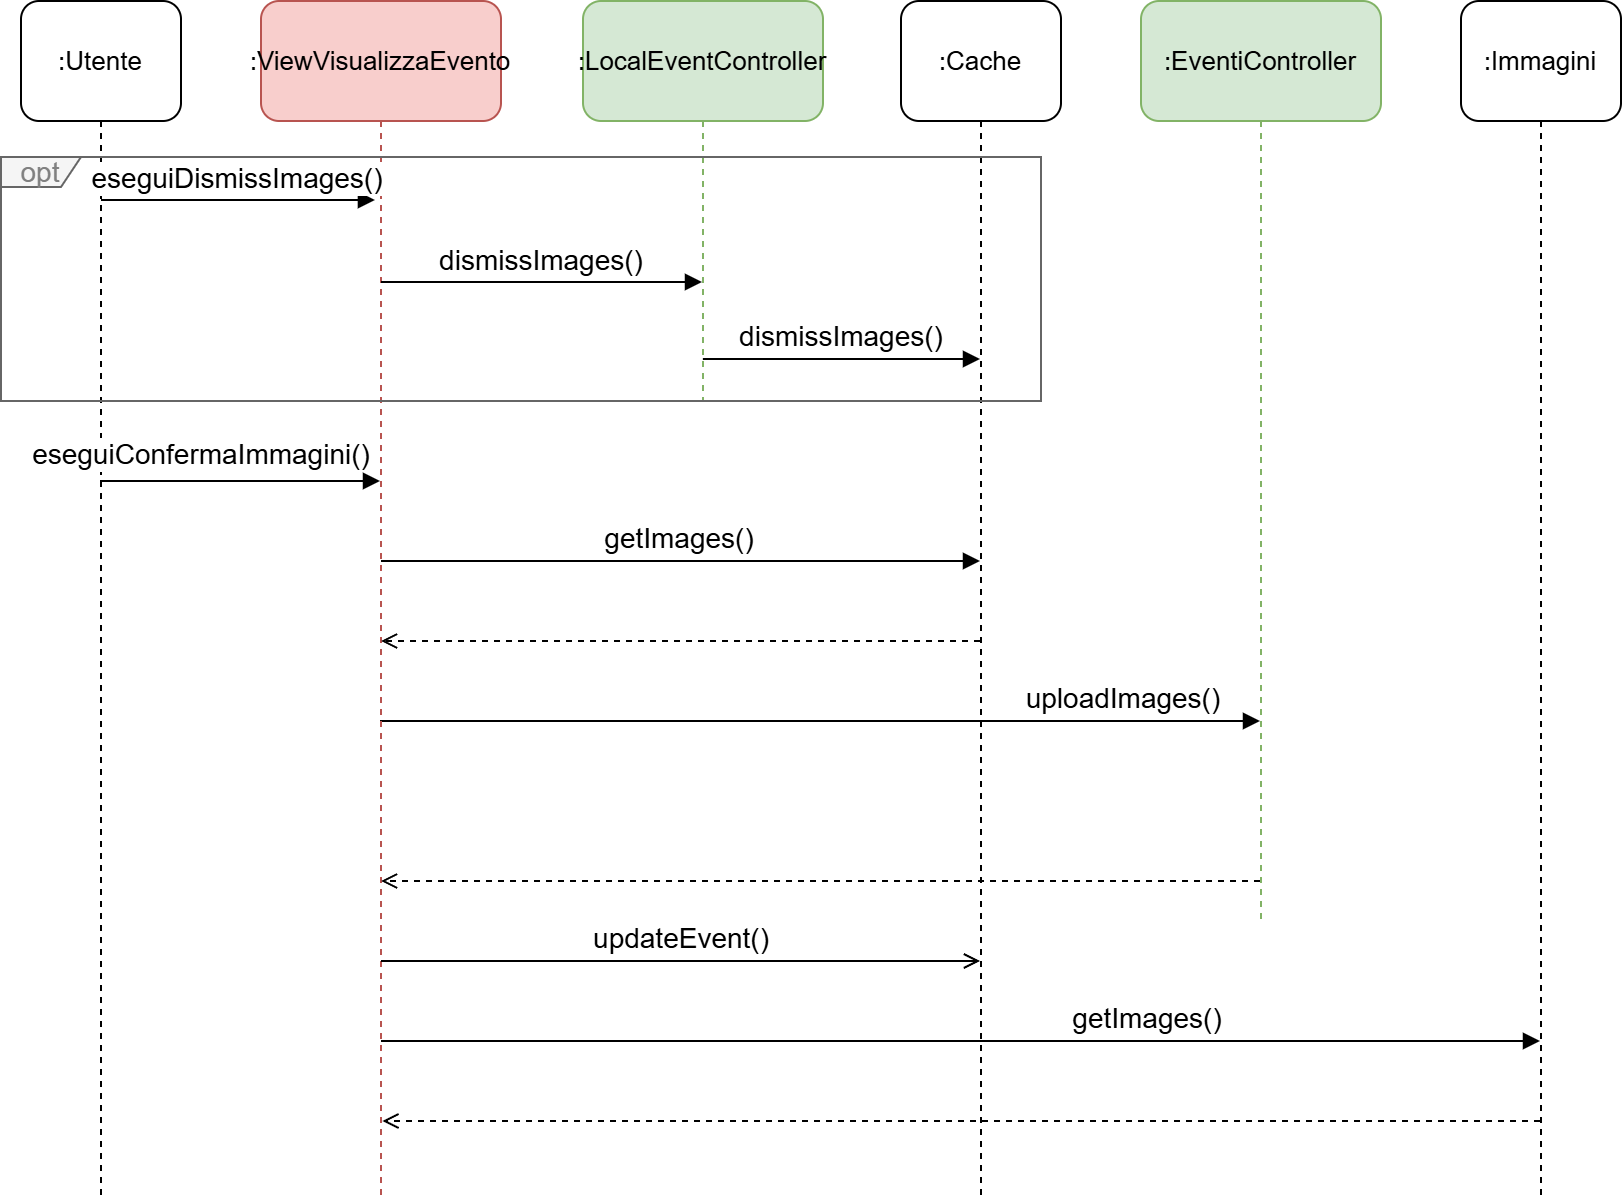
\includegraphics[width=\textwidth]{PIConfermaImmagini1.png}
\end{figure}

\textbf{Diagramma di Sequenza: Conferma Immagini - Server}
\begin{figure}[h!]
    \centering
    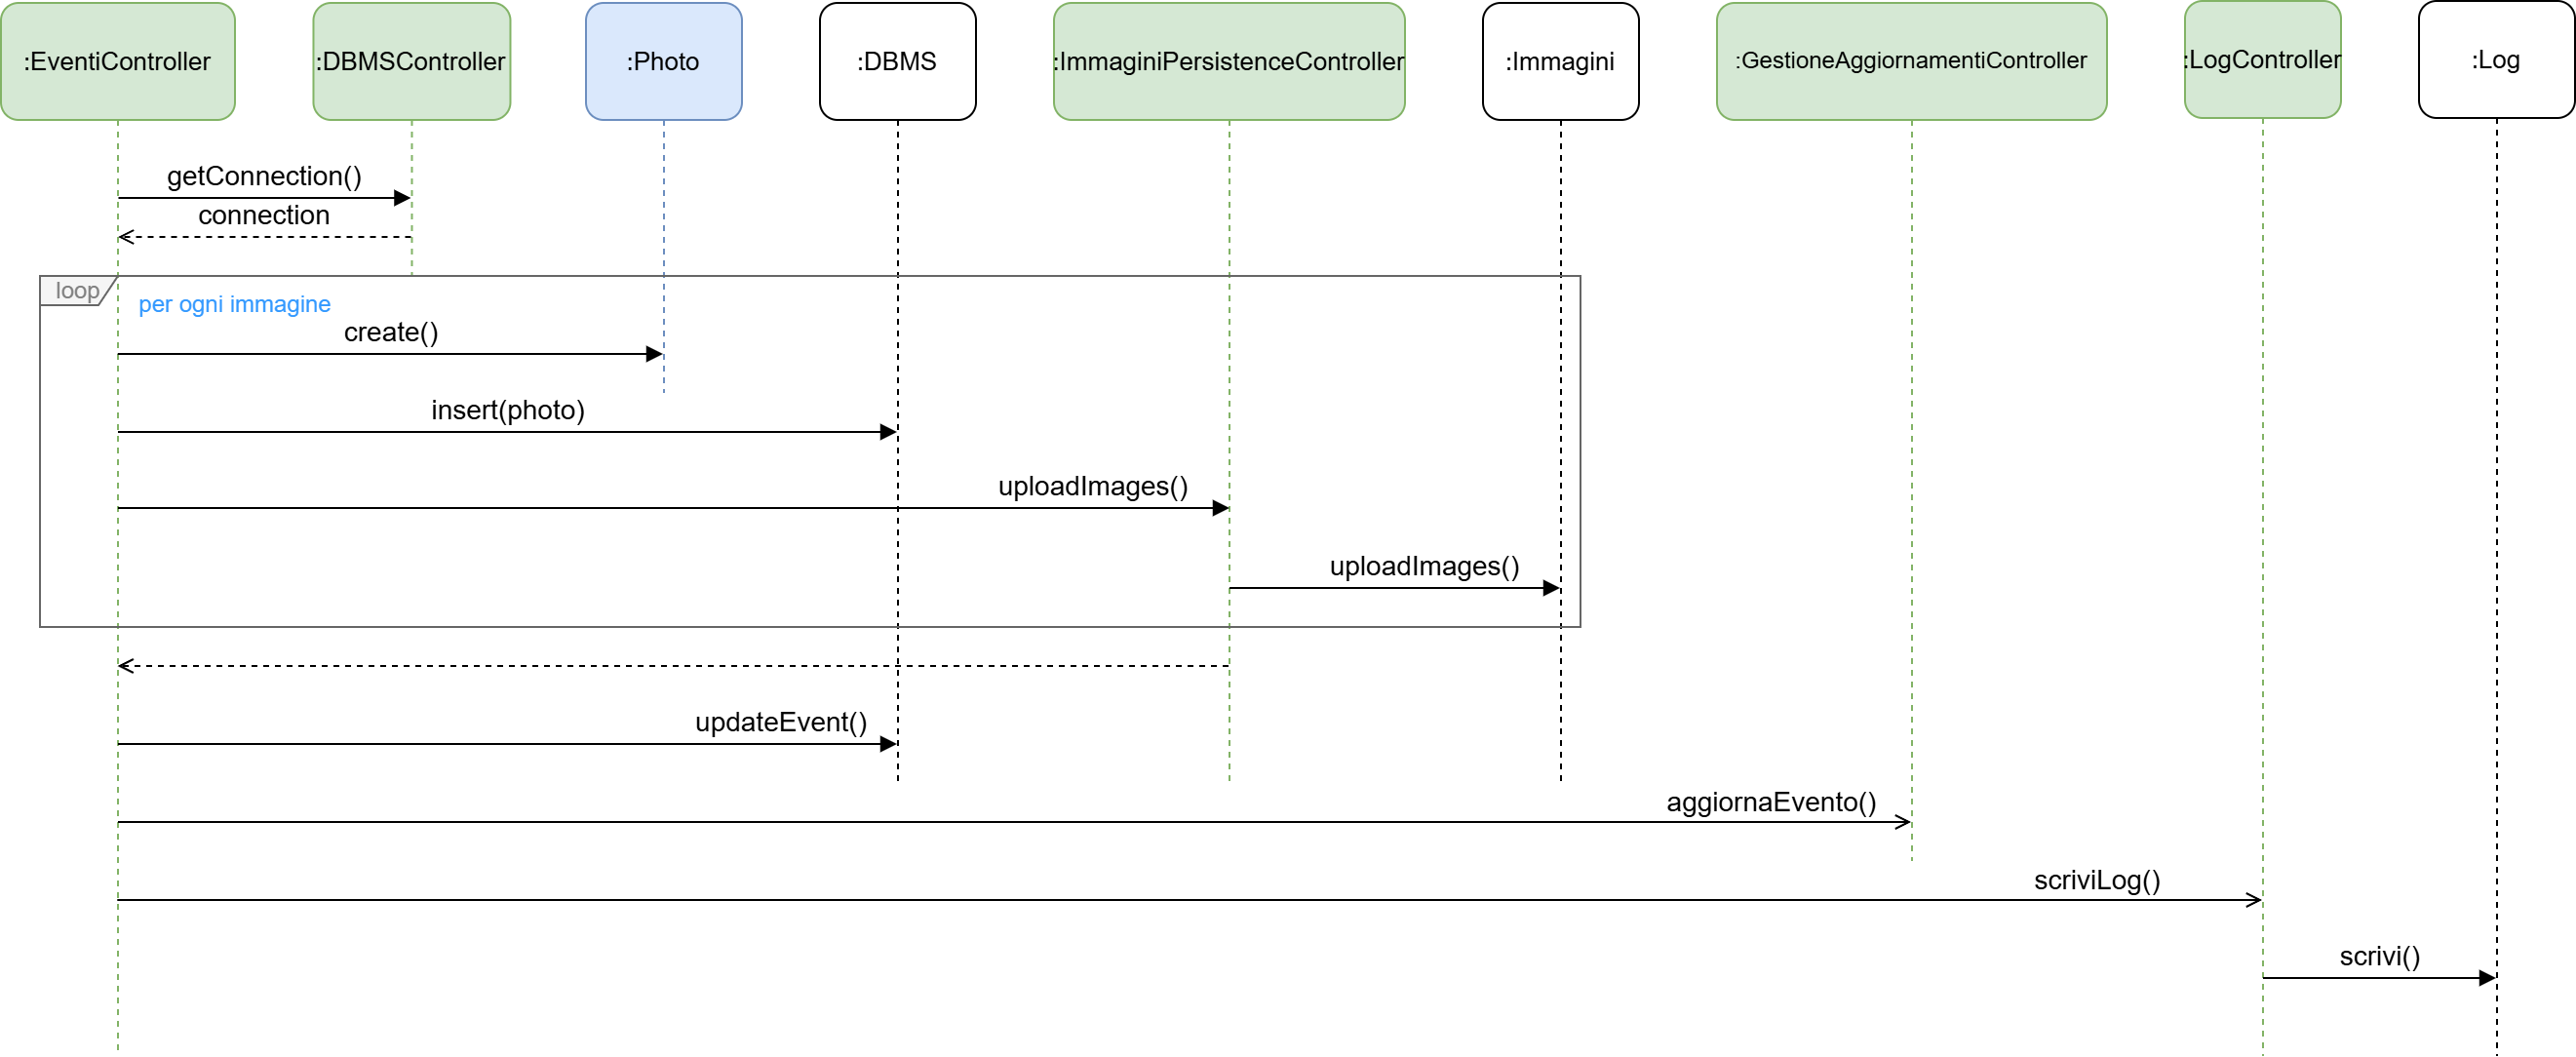
\includegraphics[width=\textwidth]{PIConfermaImmagini2.png}
\end{figure}
\clearpage

\textbf{Diagramma di Sequenza: Condividi Evento ai Gruppi}
\begin{figure}[h!]
    \centering
    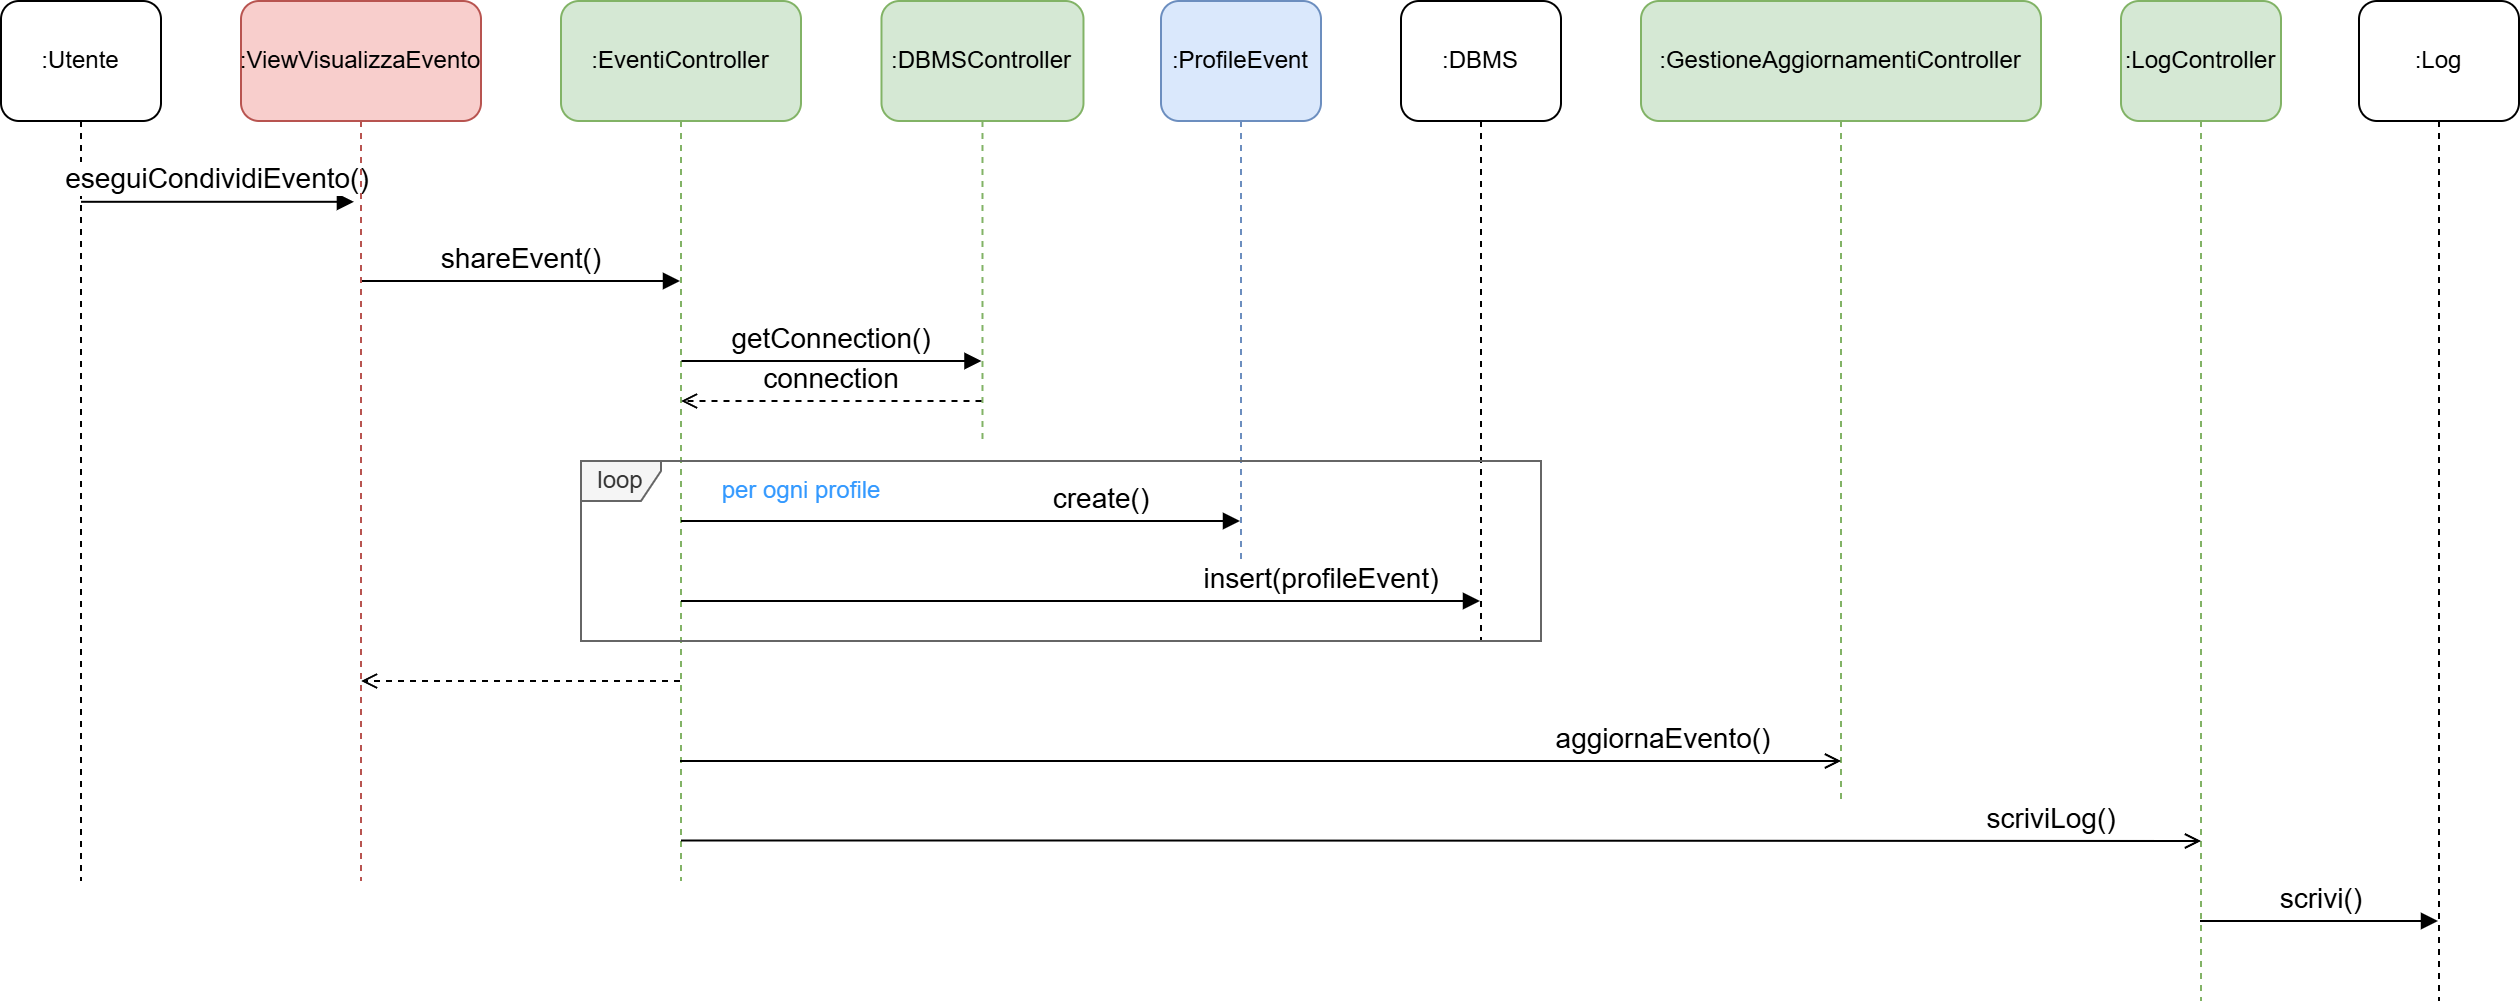
\includegraphics[width=\textwidth]{PICondividiEventoAiGruppi.png}
\end{figure}

\textbf{Diagramma di Sequenza: Cerca profili}
\begin{figure}[h!]
    \centering
    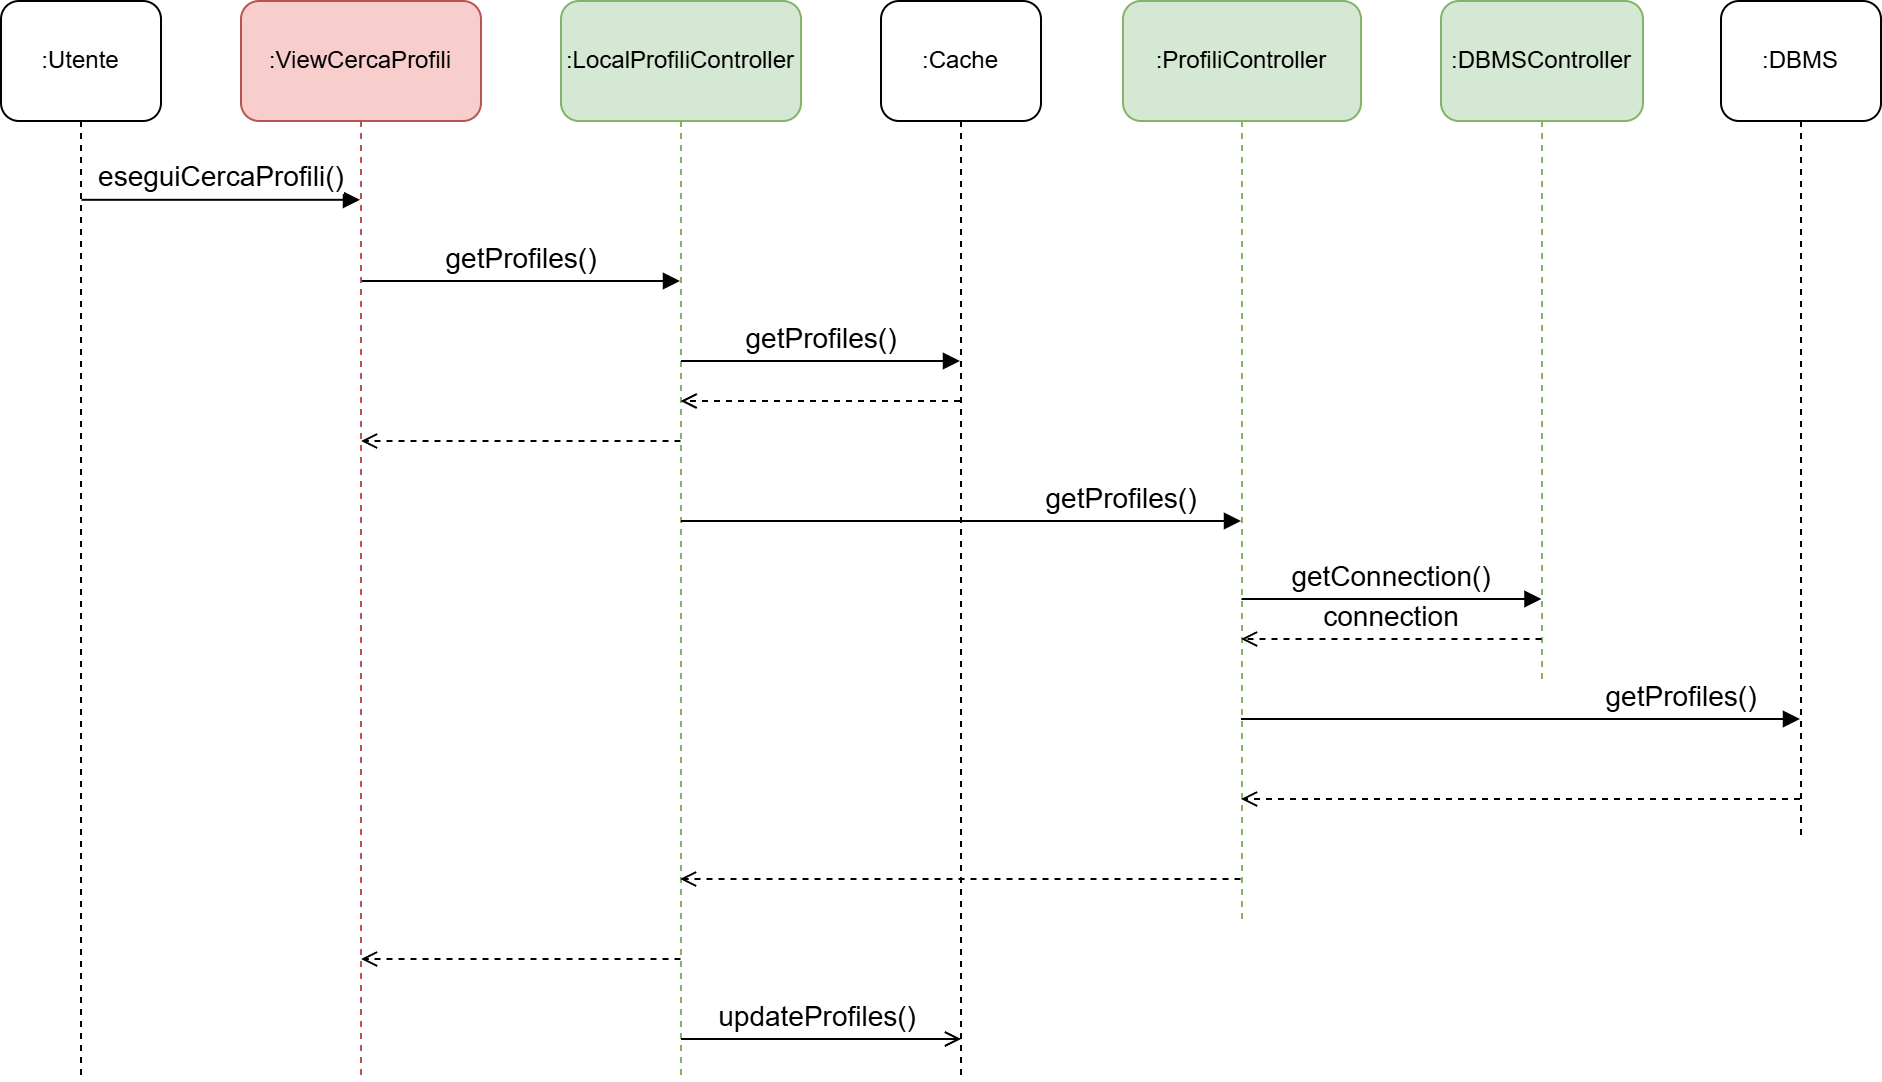
\includegraphics[width=\textwidth]{PICercaProfili.png}
\end{figure}

%\adjustbox{valign=c, width=0.95\textheight, angle=90}{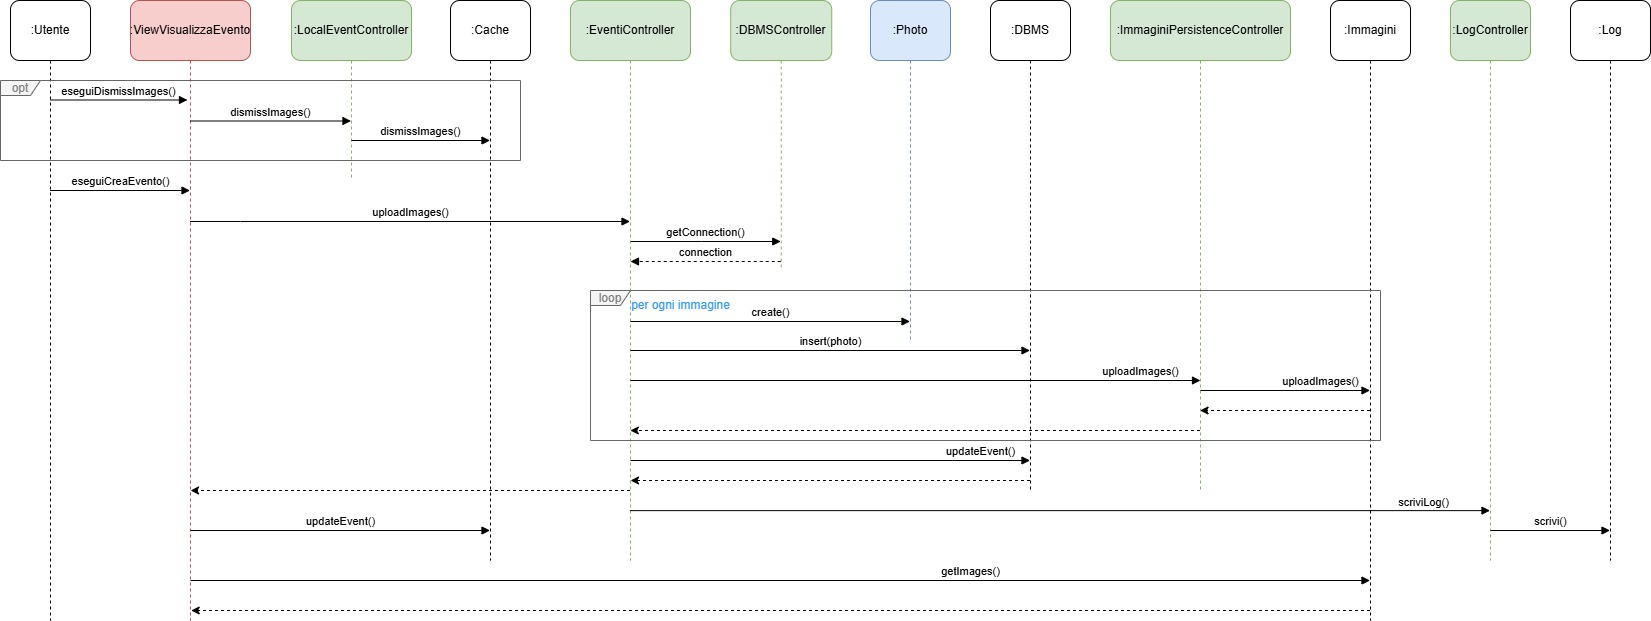
\includegraphics{PIConfermaImmagini.png}}

\clearpage


\subsection{Progettazione della persistenza}

\subsubsection{Diagramma E-R}

\begin{figure}[h!]
    \begin{center}
        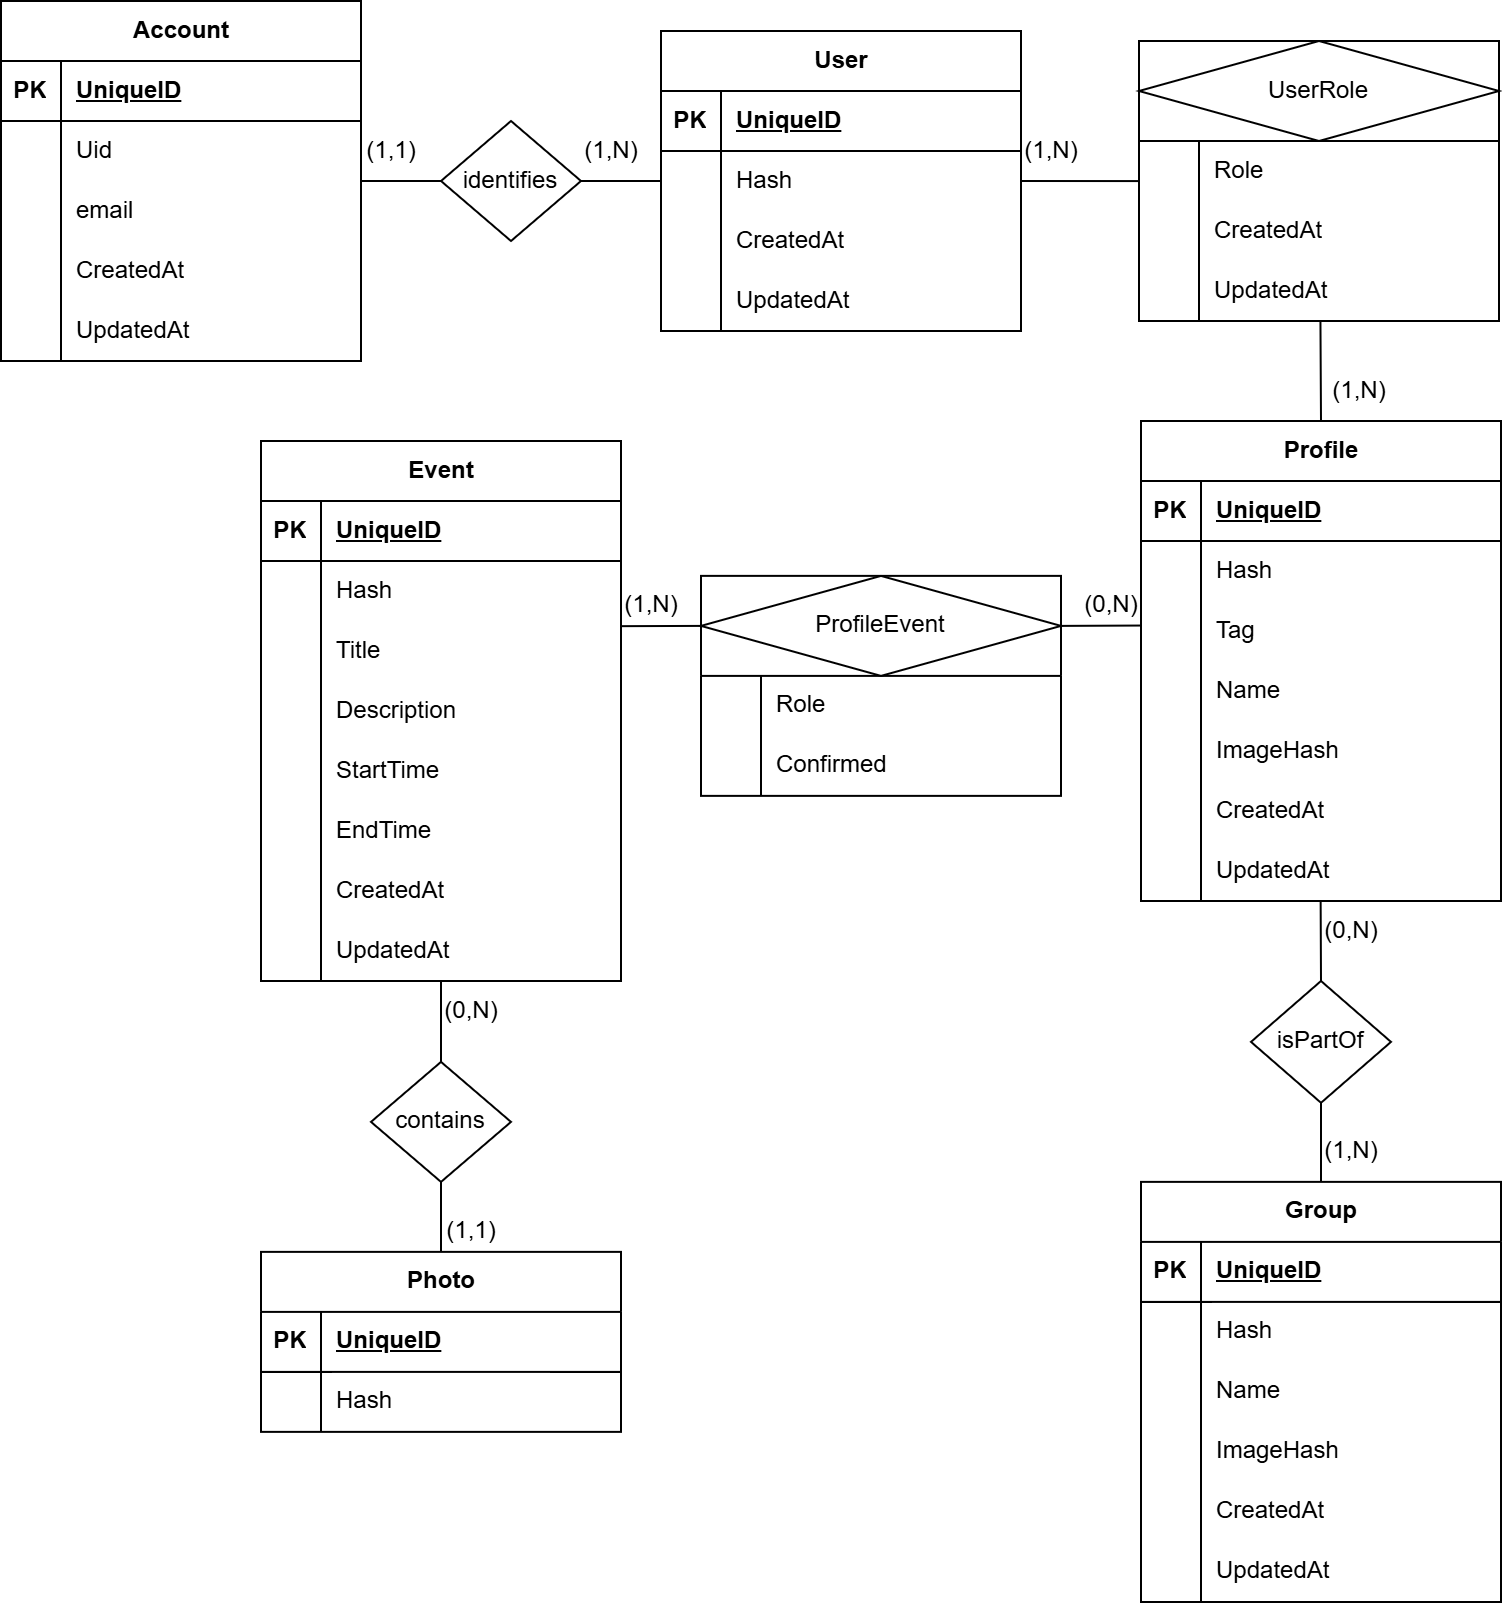
\includegraphics[width=\textwidth]{ProgettoDiagrammaER.png}
    \end{center}
\end{figure}

Come si può notare, il diagramma E-R della persistenza segue precisamente la struttura del modello del dominio mostrato precedentemente.
La differenza sta nelle associazioni, che presumibilmente in fase di progettazione logica ed implementazione del database verranno concretizzate in classi di associazione,
si avranno quindi due tabelle ulteriori (\texttt{ProfileEvent} e \texttt{UserRole}) per modellare le associazioni.

\subsubsection{Formato dei file di log}

Il formato del file di log su cui il sistema terrà traccia delle operazioni
sarà il seguente:\\

Esempio: File \texttt{/var/log/wyd.log}\\

\texttt{\$ Data - Ora - Operazione - Descrizione - ID utente}\\
\textbf{Nota}: l'ID utente è l'identificativo dell'esecutore di tale operazione.
\newpage

%\subsection{Progettazione del collaudo}

%\vspace{2em}

%\subsection{Progettazione per il deployment}

%\newpage

\subsection{Deployment}

\subsubsection{Artefatti}

\begin{figure}[h!]
    \begin{center}
        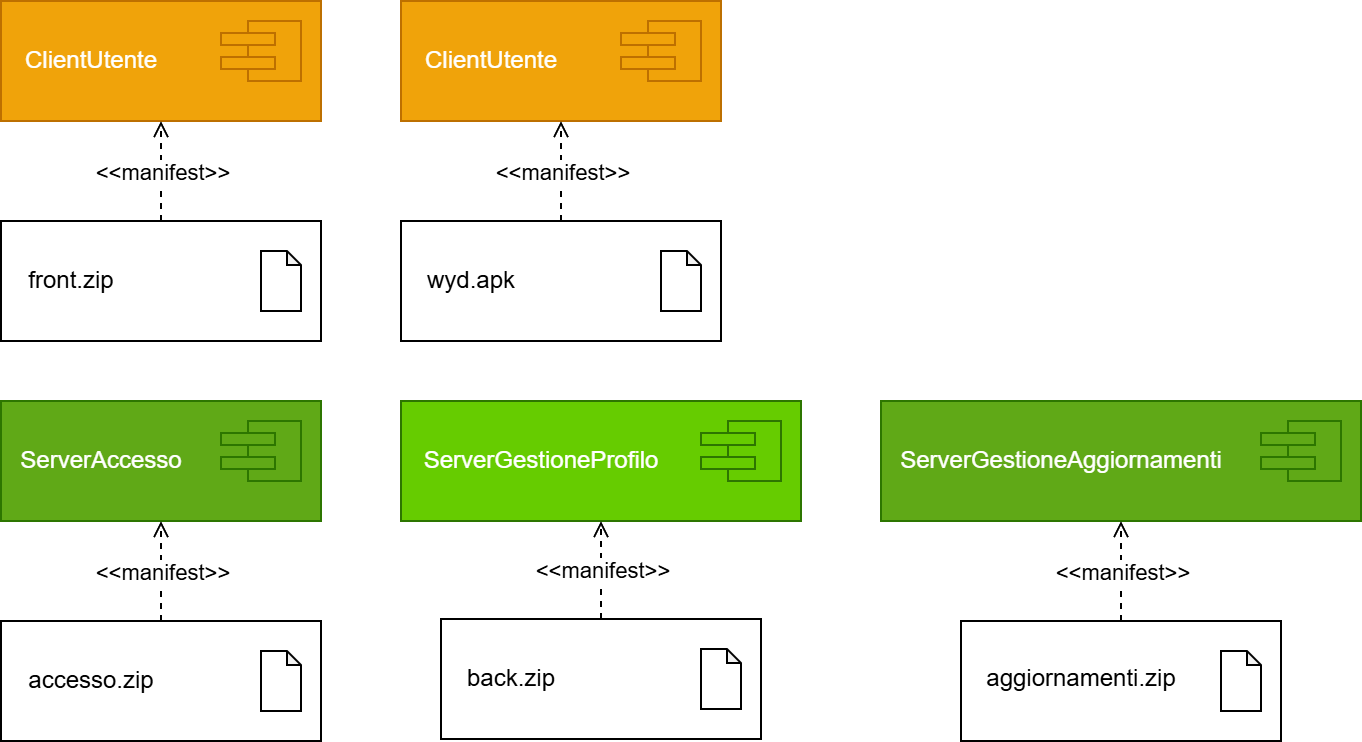
\includegraphics[height=0.25\textheight]{ProgettoDeploymentArtefatti.png}
    \end{center}
\end{figure}

\subsubsection{Deployment Type-Level}

\begin{figure}[h!]
    \begin{center}
        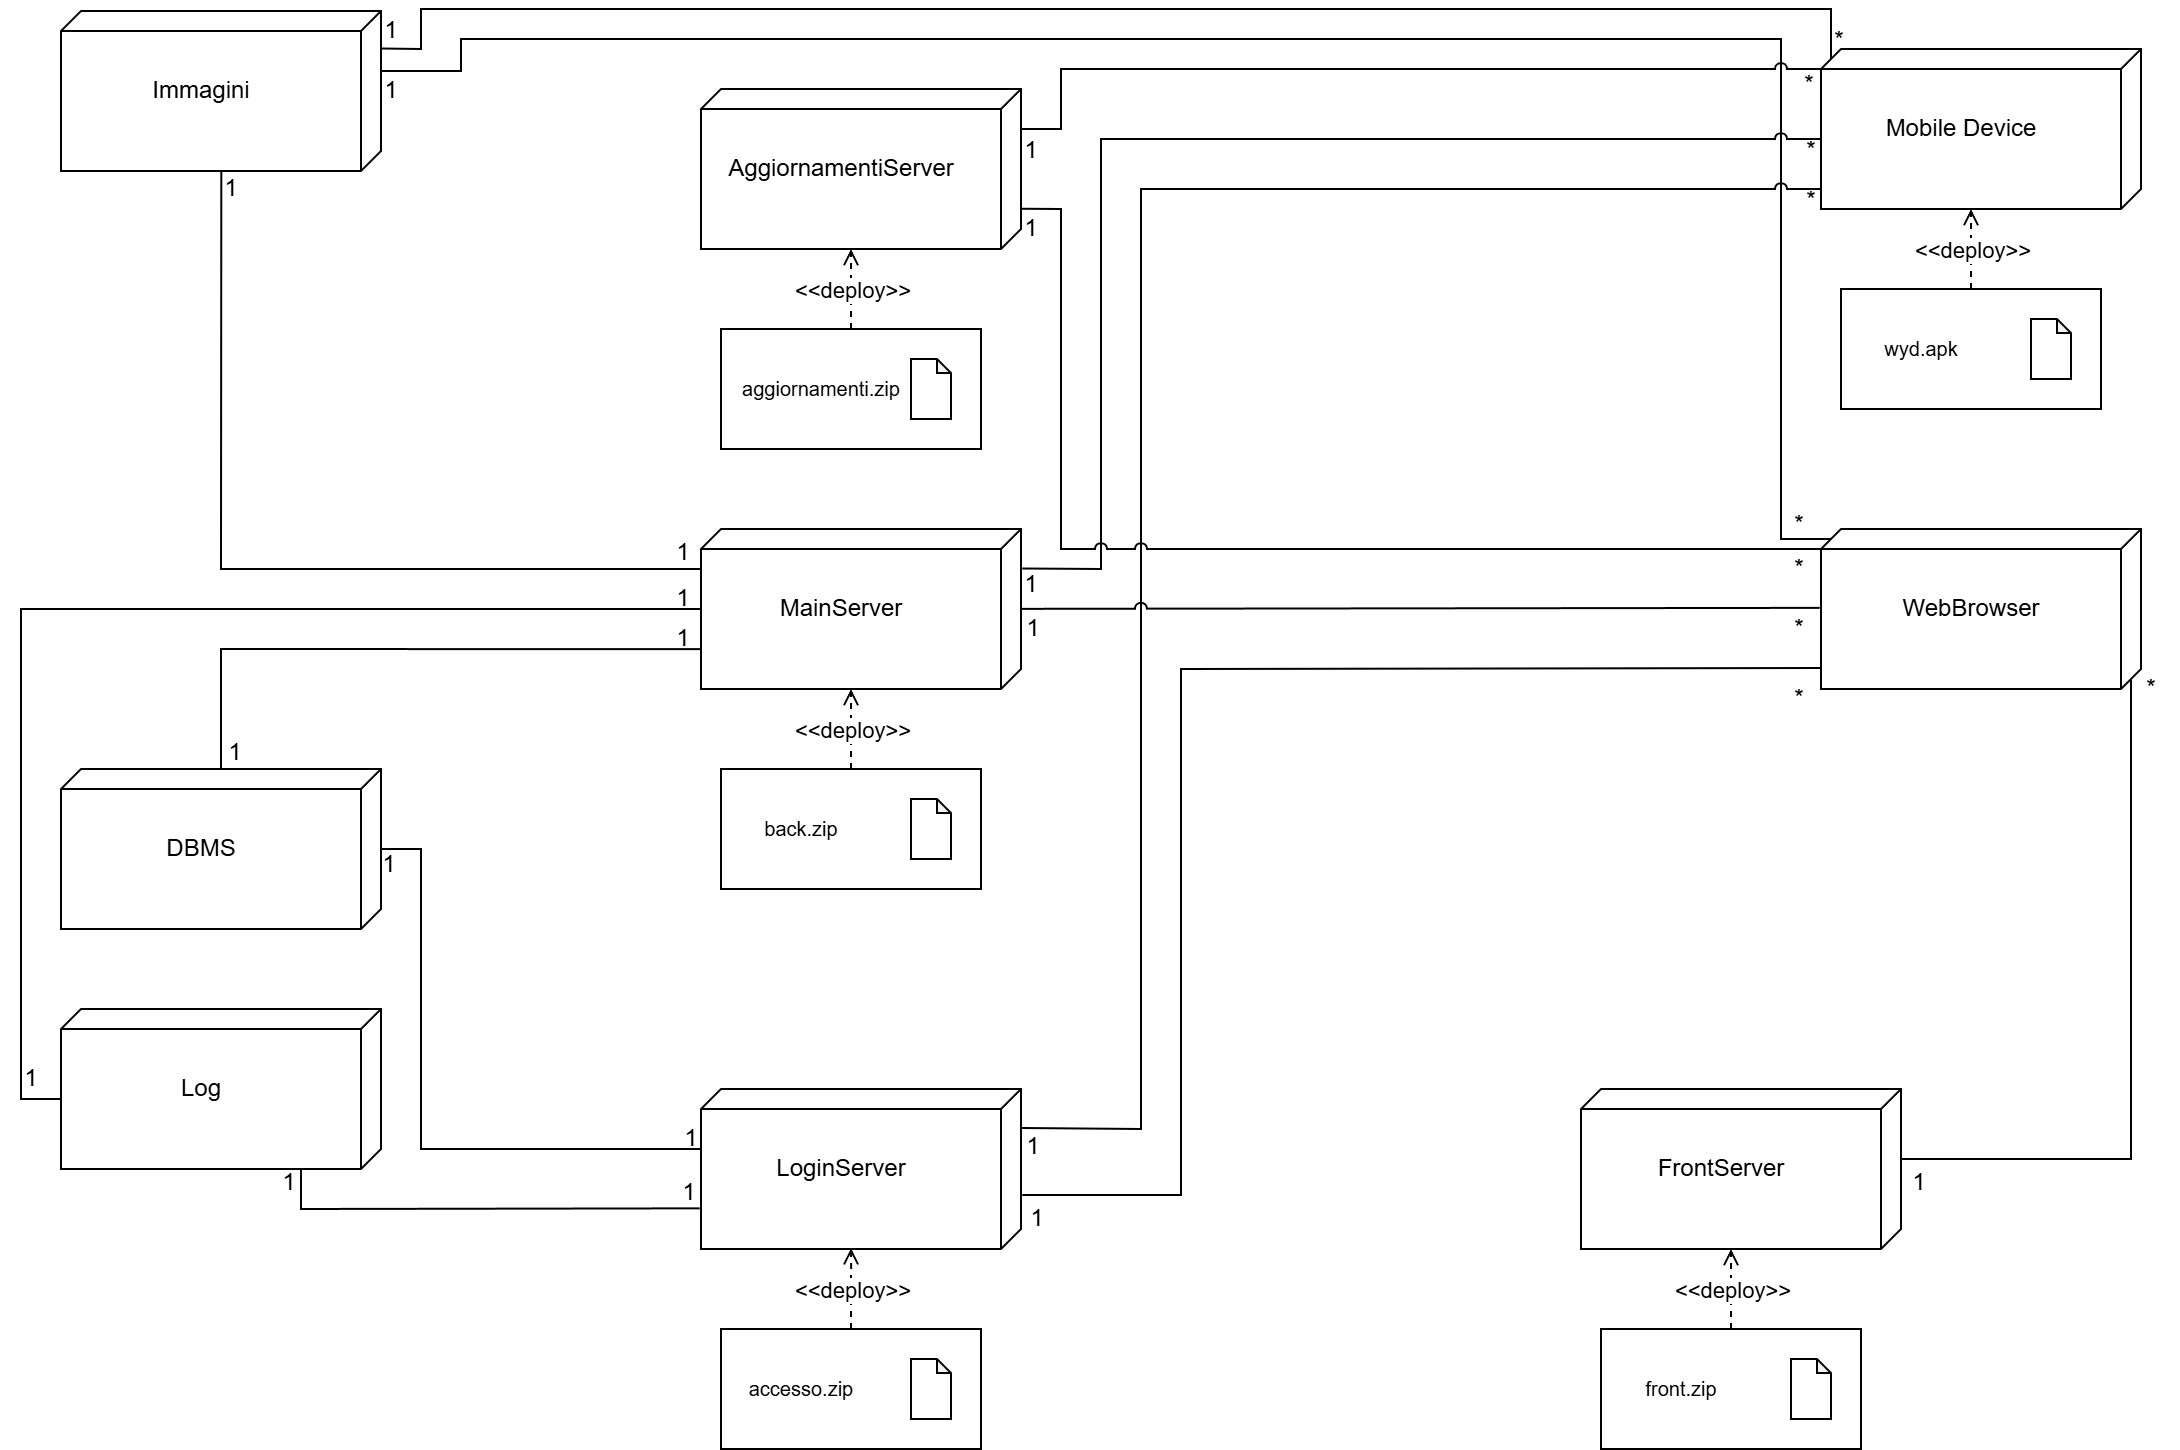
\includegraphics[height=0.45\textheight]{ProgettoDeploymentTypeLevel.png}
    \end{center}
\end{figure}
